% Options for packages loaded elsewhere
\PassOptionsToPackage{unicode}{hyperref}
\PassOptionsToPackage{hyphens}{url}
\PassOptionsToPackage{dvipsnames,svgnames*,x11names*}{xcolor}
%
\documentclass[
  12pt,
  portuguese,
]{report}
\usepackage{lmodern}
\usepackage{amsmath}
\usepackage{ifxetex,ifluatex}
\ifnum 0\ifxetex 1\fi\ifluatex 1\fi=0 % if pdftex
  \usepackage[T1]{fontenc}
  \usepackage[utf8]{inputenc}
  \usepackage{textcomp} % provide euro and other symbols
  \usepackage{amssymb}
\else % if luatex or xetex
  \usepackage{unicode-math}
  \defaultfontfeatures{Scale=MatchLowercase}
  \defaultfontfeatures[\rmfamily]{Ligatures=TeX,Scale=1}
\fi
% Use upquote if available, for straight quotes in verbatim environments
\IfFileExists{upquote.sty}{\usepackage{upquote}}{}
\IfFileExists{microtype.sty}{% use microtype if available
  \usepackage[]{microtype}
  \UseMicrotypeSet[protrusion]{basicmath} % disable protrusion for tt fonts
}{}
\makeatletter
\@ifundefined{KOMAClassName}{% if non-KOMA class
  \IfFileExists{parskip.sty}{%
    \usepackage{parskip}
  }{% else
    \setlength{\parindent}{0pt}
    \setlength{\parskip}{6pt plus 2pt minus 1pt}}
}{% if KOMA class
  \KOMAoptions{parskip=half}}
\makeatother
\usepackage{xcolor}
\IfFileExists{xurl.sty}{\usepackage{xurl}}{} % add URL line breaks if available
\IfFileExists{bookmark.sty}{\usepackage{bookmark}}{\usepackage{hyperref}}
\hypersetup{
  pdftitle={Criminalidade em São Paulo},
  pdfauthor={Grupo 3},
  pdflang={pt},
  colorlinks=true,
  linkcolor=Maroon,
  filecolor=Maroon,
  citecolor=Blue,
  urlcolor=Blue,
  pdfcreator={LaTeX via pandoc}}
\urlstyle{same} % disable monospaced font for URLs
\usepackage{color}
\usepackage{fancyvrb}
\newcommand{\VerbBar}{|}
\newcommand{\VERB}{\Verb[commandchars=\\\{\}]}
\DefineVerbatimEnvironment{Highlighting}{Verbatim}{commandchars=\\\{\}}
% Add ',fontsize=\small' for more characters per line
\usepackage{framed}
\definecolor{shadecolor}{RGB}{248,248,248}
\newenvironment{Shaded}{\begin{snugshade}}{\end{snugshade}}
\newcommand{\AlertTok}[1]{\textcolor[rgb]{0.94,0.16,0.16}{#1}}
\newcommand{\AnnotationTok}[1]{\textcolor[rgb]{0.56,0.35,0.01}{\textbf{\textit{#1}}}}
\newcommand{\AttributeTok}[1]{\textcolor[rgb]{0.77,0.63,0.00}{#1}}
\newcommand{\BaseNTok}[1]{\textcolor[rgb]{0.00,0.00,0.81}{#1}}
\newcommand{\BuiltInTok}[1]{#1}
\newcommand{\CharTok}[1]{\textcolor[rgb]{0.31,0.60,0.02}{#1}}
\newcommand{\CommentTok}[1]{\textcolor[rgb]{0.56,0.35,0.01}{\textit{#1}}}
\newcommand{\CommentVarTok}[1]{\textcolor[rgb]{0.56,0.35,0.01}{\textbf{\textit{#1}}}}
\newcommand{\ConstantTok}[1]{\textcolor[rgb]{0.00,0.00,0.00}{#1}}
\newcommand{\ControlFlowTok}[1]{\textcolor[rgb]{0.13,0.29,0.53}{\textbf{#1}}}
\newcommand{\DataTypeTok}[1]{\textcolor[rgb]{0.13,0.29,0.53}{#1}}
\newcommand{\DecValTok}[1]{\textcolor[rgb]{0.00,0.00,0.81}{#1}}
\newcommand{\DocumentationTok}[1]{\textcolor[rgb]{0.56,0.35,0.01}{\textbf{\textit{#1}}}}
\newcommand{\ErrorTok}[1]{\textcolor[rgb]{0.64,0.00,0.00}{\textbf{#1}}}
\newcommand{\ExtensionTok}[1]{#1}
\newcommand{\FloatTok}[1]{\textcolor[rgb]{0.00,0.00,0.81}{#1}}
\newcommand{\FunctionTok}[1]{\textcolor[rgb]{0.00,0.00,0.00}{#1}}
\newcommand{\ImportTok}[1]{#1}
\newcommand{\InformationTok}[1]{\textcolor[rgb]{0.56,0.35,0.01}{\textbf{\textit{#1}}}}
\newcommand{\KeywordTok}[1]{\textcolor[rgb]{0.13,0.29,0.53}{\textbf{#1}}}
\newcommand{\NormalTok}[1]{#1}
\newcommand{\OperatorTok}[1]{\textcolor[rgb]{0.81,0.36,0.00}{\textbf{#1}}}
\newcommand{\OtherTok}[1]{\textcolor[rgb]{0.56,0.35,0.01}{#1}}
\newcommand{\PreprocessorTok}[1]{\textcolor[rgb]{0.56,0.35,0.01}{\textit{#1}}}
\newcommand{\RegionMarkerTok}[1]{#1}
\newcommand{\SpecialCharTok}[1]{\textcolor[rgb]{0.00,0.00,0.00}{#1}}
\newcommand{\SpecialStringTok}[1]{\textcolor[rgb]{0.31,0.60,0.02}{#1}}
\newcommand{\StringTok}[1]{\textcolor[rgb]{0.31,0.60,0.02}{#1}}
\newcommand{\VariableTok}[1]{\textcolor[rgb]{0.00,0.00,0.00}{#1}}
\newcommand{\VerbatimStringTok}[1]{\textcolor[rgb]{0.31,0.60,0.02}{#1}}
\newcommand{\WarningTok}[1]{\textcolor[rgb]{0.56,0.35,0.01}{\textbf{\textit{#1}}}}
\usepackage{longtable,booktabs}
% Correct order of tables after \paragraph or \subparagraph
\usepackage{etoolbox}
\makeatletter
\patchcmd\longtable{\par}{\if@noskipsec\mbox{}\fi\par}{}{}
\makeatother
% Allow footnotes in longtable head/foot
\IfFileExists{footnotehyper.sty}{\usepackage{footnotehyper}}{\usepackage{footnote}}
\makesavenoteenv{longtable}
\usepackage{graphicx}
\makeatletter
\def\maxwidth{\ifdim\Gin@nat@width>\linewidth\linewidth\else\Gin@nat@width\fi}
\def\maxheight{\ifdim\Gin@nat@height>\textheight\textheight\else\Gin@nat@height\fi}
\makeatother
% Scale images if necessary, so that they will not overflow the page
% margins by default, and it is still possible to overwrite the defaults
% using explicit options in \includegraphics[width, height, ...]{}
\setkeys{Gin}{width=\maxwidth,height=\maxheight,keepaspectratio}
% Set default figure placement to htbp
\makeatletter
\def\fps@figure{htbp}
\makeatother
\setlength{\emergencystretch}{3em} % prevent overfull lines
\providecommand{\tightlist}{%
  \setlength{\itemsep}{0pt}\setlength{\parskip}{0pt}}
\setcounter{secnumdepth}{5}
\ifxetex
  % Load polyglossia as late as possible: uses bidi with RTL langages (e.g. Hebrew, Arabic)
  \usepackage{polyglossia}
  \setmainlanguage[]{portuguese}
\else
  \usepackage[shorthands=off,main=portuguese]{babel}
\fi
\ifluatex
  \usepackage{selnolig}  % disable illegal ligatures
\fi
\newlength{\cslhangindent}
\setlength{\cslhangindent}{1.5em}
\newlength{\csllabelwidth}
\setlength{\csllabelwidth}{3em}
\newenvironment{CSLReferences}[3] % #1 hanging-ident, #2 entry spacing
 {% don't indent paragraphs
  \setlength{\parindent}{0pt}
  % turn on hanging indent if param 1 is 1
  \ifodd #1 \everypar{\setlength{\hangindent}{\cslhangindent}}\ignorespaces\fi
  % set entry spacing
  \ifnum #2 > 0
  \setlength{\parskip}{#2\baselineskip}
  \fi
 }%
 {}
\usepackage{calc} % for \widthof, \maxof
\newcommand{\CSLBlock}[1]{#1\hfill\break}
\newcommand{\CSLLeftMargin}[1]{\parbox[t]{\maxof{\widthof{#1}}{\csllabelwidth}}{#1}}
\newcommand{\CSLRightInline}[1]{\parbox[t]{\linewidth}{#1}}
\newcommand{\CSLIndent}[1]{\hspace{\cslhangindent}#1}

\title{Criminalidade em São Paulo}
\author{Grupo 3}
\date{02 de dezembro de 2020}

\begin{document}
\maketitle

\listoftables
\listoffigures
\hypertarget{sobre-este-documento}{%
\chapter*{Sobre este documento}\label{sobre-este-documento}}
\addcontentsline{toc}{chapter}{Sobre este documento}

Este relatório foi produzido em \emph{RMarkdown}. As análises foram desenvolvidas como trabalho final da disciplina MAE5904/MAE0501 - Aprendizagem estatística em altas dimensões, ministrada pela professora Florencia Leonardi no segundo semestre de 2020.

Os integrantes do grupo responsável por este relatório são:

\begin{itemize}
\tightlist
\item
  Lucas de Miranda Oliveira
\item
  Pedro Henrique Sebe Rodrigues
\item
  Renata Massami Hirota
\item
  Rodolfo Riani Sundfeld
\item
  Rubens Santos Andrade Filho
\end{itemize}

\hypertarget{introducao}{%
\chapter{Introdução}\label{introducao}}

O Brasil tem a segunda maior taxa de homicídios da América do Sul, segundo relatório das Nações Unidas em 2017, e ocupa a 12ª posição no ranking global de violência, com uma taxa de 30,5 homicídios a cada 100.000 habitantes.

Em 2016, a Organização para a Cooperação e Desenvolvimento Econômico (OCDE) divulgou que as vítimas de assaltos no Brasil, nos últimos 12 meses da pesquisa, foram de 7,9\% dos entrevistados, quase o dobro da média dos países em que a pesquisa foi realizada. Este preocupante quadro mostra a situação da violência e a necessidade de políticas públicas adequadas para segurança pública.

\hypertarget{objetivo}{%
\section{Objetivo}\label{objetivo}}

A partir de dados de boletins de ocorrência (BO) da Secretaria de Seguraça Pública (SSP) do estado de São Paulo, o objetivo deste estudo é prever o horário do crime de acordo com algumas características, por exemplo, localização, sexo da vítima, cor da vítma, entre outros.

Dessa forma, visa-se identificar quais os horários das ocorrências de acordo com a tipologia do crime e assim fornecer insights para o policiamento.

\hypertarget{questuxf5es-norteadoras}{%
\section{Questões Norteadoras}\label{questuxf5es-norteadoras}}

O projeto dedica-se à análise dos boletins de ocorrência da Secretaria de Segurança Pública de São Paulo, endereçando os pontos principais abaixo.

\begin{itemize}
\tightlist
\item
  Em que períodos do dia ocorrem mais crimes?
\item
  Existe relação entre localização e horário?
\item
  Que características das ocorrências são relacionadas ao período?
\end{itemize}

A pesquisa utilizou como base tais questões, que orientam a análise dos dados, para chegar a conclusões acerca de aplicações práticas e orientações a respeito, por exemplo, do policiamento na cidade de São Paulo para o combate à criminalidade.

\hypertarget{organizauxe7uxe3o-do-trabalho}{%
\section{Organização do trabalho}\label{organizauxe7uxe3o-do-trabalho}}

O presente relatório foi organizado em três capítulos, além desta introdução. No Capítulo \ref{metodologia}, apresentamos as decisões metodológicas e organização dos dados de BOs. No Capítulo \ref{resultados}, apresentamos os principais resultados dos métodos utilizados, organizados de acordo com cada método. No Capítulo \ref{conclusoes}, apresentamos as considerações finais e sugestões.

\hypertarget{metodologia}{%
\chapter{Metodologia}\label{metodologia}}

No Capítulo \ref{introducao}, citamos brevemente algumas das variáveis que podem ser de interesse na análise dos boletins de ocorrência e as principais perguntas. Neste capítulo, apresentamos o conjunto de dados e os procedimento de tratamento e análise realizados para atingir nossos objetivos.

\hypertarget{fonte-dos-dados}{%
\section{Fonte dos dados}\label{fonte-dos-dados}}

A base de dados que será trabalhada refere-se a boletins de ocorrência na Grande São Paulo, disponível em \href{https://www.kaggle.com/inquisitivecrow/crime-data-in-brazil}{Crime Data in Brazil - Kaggle}.

Abaixo estão listadas todas as variáveis e suas respectivas descrições, segundo dicionário de dados fornecido no mesmo repositório.

\begin{tabular}{l|l}
\hline
Variável & Descrição\\
\hline
ID\_DELEGACIA & Código da delegacia responsável pelo registro da ocorrencia\\
\hline
NOME\_DEPARTAMENTO & Departamento responsável pelo registro\\
\hline
NOME\_SECCIONAL & Delegacia Seccional responsável pelo registro\\
\hline
NOME\_DELEGACIA & Delegacia responsável pelo registro\\
\hline
CIDADE & Cidade de Registro\\
\hline
ANO\_BO & Ano da ocorrencia\\
\hline
NUM\_BO & Número do BO\\
\hline
NOME\_DEPARTAMENTO\_CIRC & Departamento de Circunscrição\\
\hline
NOME\_SECCIONAL\_CIRC & Seccional de Circunscrição\\
\hline
NOME\_DELEGACIA\_CIRC & Delegacia de Circunscrição\\
\hline
NOME\_MUNICIPIO\_CIRC & Município de Circunscrição\\
\hline
DESCR\_TIPO\_BO & Tipo de Documento\\
\hline
DATA\_OCORRENCIA\_BO & Data da Ocorrência\\
\hline
HORA\_OCORRENCIA\_BO & Hora da Ocorrência\\
\hline
DATAHORA\_COMUNICACAO\_BO & Data Hora da Comunicação da Ocorrência\\
\hline
FLAG\_STATUS & Status da Ocorrência\\
\hline
RUBRICA & Natureza jurídica da ocorrência\\
\hline
DESCR\_CONDUTA & Conduta na Ocorrência\\
\hline
DESDOBRAMENTO & Desdobramento na Ocorrência\\
\hline
DESCR\_TIPOLOCAL & Tipo de Local\\
\hline
DESCR\_SUBTIPOLOCAL & Descrição do subTipo de local\\
\hline
LOGRADOURO & Logradouro dos fatos\\
\hline
NUMERO\_LOGRADOURO & Numero do Logradouro dos fatos\\
\hline
LATITUDE & Latitude da Ocorrência\\
\hline
LONGITUDE & Longitude da Ocorrência\\
\hline
DESCR\_TIPO\_PESSOA & Qualificação do envolvido na ocorrência\\
\hline
FLAG\_VITIMA\_FATAL & Condição do Autor / Vítma na corrência\\
\hline
SEXO\_PESSOA & Sexo\\
\hline
IDADE\_PESSOA & Idade\\
\hline
COR\_CUTIS & Cor da Pele\\
\hline
\end{tabular}

\hypertarget{filtros-de-escopo-e-tratamento-dos-dados}{%
\section{Filtros de escopo e tratamento dos dados}\label{filtros-de-escopo-e-tratamento-dos-dados}}

Algumas variáveis foram tratadas para refletir sua natureza real, como, por exemplo, datas e horários.

\begin{Shaded}
\begin{Highlighting}[]
\NormalTok{df }\OtherTok{\textless{}{-}} \FunctionTok{read.csv}\NormalTok{(}\StringTok{\textquotesingle{}RDO\_3.csv\textquotesingle{}}\NormalTok{)}
\NormalTok{df}\SpecialCharTok{$}\NormalTok{DATA\_OCORRENCIA\_BO }\OtherTok{\textless{}{-}} \FunctionTok{as.Date}\NormalTok{(df}\SpecialCharTok{$}\NormalTok{DATA\_OCORRENCIA\_BO,}\AttributeTok{format=}\StringTok{"\%d/\%m/\%Y"}\NormalTok{)}
\NormalTok{df}\SpecialCharTok{$}\NormalTok{HORA\_OCORRENCIA\_BO }\OtherTok{\textless{}{-}}\NormalTok{ lubridate}\SpecialCharTok{::}\FunctionTok{hour}\NormalTok{(}\FunctionTok{strptime}\NormalTok{(}\AttributeTok{x =}\NormalTok{ df}\SpecialCharTok{$}\NormalTok{HORA\_OCORRENCIA\_BO, }\AttributeTok{format =} \StringTok{"\%H:\%M"}\NormalTok{))}
\NormalTok{df}\SpecialCharTok{$}\NormalTok{IDADE\_PESSOA }\OtherTok{\textless{}{-}} \FunctionTok{as.numeric}\NormalTok{(df}\SpecialCharTok{$}\NormalTok{IDADE\_PESSOA)}
\NormalTok{df }\OtherTok{\textless{}{-}}\NormalTok{ df[}\SpecialCharTok{!}\NormalTok{(}\FunctionTok{is.na}\NormalTok{(df}\SpecialCharTok{$}\NormalTok{HORA\_OCORRENCIA\_BO) }\SpecialCharTok{|}\NormalTok{ df}\SpecialCharTok{$}\NormalTok{HORA\_OCORRENCIA\_BO}\SpecialCharTok{==}\StringTok{""}\NormalTok{), ]}
\NormalTok{df }\OtherTok{\textless{}{-}}\NormalTok{ df[(}\FunctionTok{is.na}\NormalTok{(df}\SpecialCharTok{$}\NormalTok{X) }\SpecialCharTok{|}\NormalTok{ df}\SpecialCharTok{$}\NormalTok{X}\SpecialCharTok{==}\StringTok{""}\NormalTok{), ]}
\NormalTok{df}\SpecialCharTok{$}\NormalTok{target }\OtherTok{\textless{}{-}} \FunctionTok{cut}\NormalTok{(df}\SpecialCharTok{$}\NormalTok{HORA\_OCORRENCIA\_BO, }
                 \AttributeTok{breaks =} \FunctionTok{c}\NormalTok{(}\SpecialCharTok{{-}}\FloatTok{0.5}\NormalTok{, }\FloatTok{5.5}\NormalTok{, }\FloatTok{11.5}\NormalTok{, }\FloatTok{17.5}\NormalTok{, }\FloatTok{23.5}\NormalTok{), }
                 \AttributeTok{labels =} \FunctionTok{c}\NormalTok{(}\StringTok{\textquotesingle{}4.Madrugada\textquotesingle{}}\NormalTok{, }\StringTok{\textquotesingle{}1.Manhã\textquotesingle{}}\NormalTok{, }\StringTok{\textquotesingle{}2.Tarde\textquotesingle{}}\NormalTok{, }\StringTok{\textquotesingle{}3.Noite\textquotesingle{}}\NormalTok{))}
\NormalTok{df}\SpecialCharTok{$}\NormalTok{LATITUDE }\OtherTok{\textless{}{-}} \FunctionTok{as.numeric}\NormalTok{(df}\SpecialCharTok{$}\NormalTok{LATITUDE)}
\NormalTok{df}\SpecialCharTok{$}\NormalTok{LONGITUDE }\OtherTok{\textless{}{-}} \FunctionTok{as.numeric}\NormalTok{(df}\SpecialCharTok{$}\NormalTok{LONGITUDE)}
\NormalTok{locations\_df }\OtherTok{\textless{}{-}}\NormalTok{ df[,}\FunctionTok{c}\NormalTok{(}\StringTok{\textquotesingle{}LATITUDE\textquotesingle{}}\NormalTok{, }\StringTok{\textquotesingle{}LONGITUDE\textquotesingle{}}\NormalTok{, }\StringTok{\textquotesingle{}target\textquotesingle{}}\NormalTok{)]}
\NormalTok{locations\_df }\OtherTok{\textless{}{-}}\NormalTok{ locations\_df[}\SpecialCharTok{!}\NormalTok{(}\FunctionTok{is.na}\NormalTok{(df}\SpecialCharTok{$}\NormalTok{LATITUDE)), ]}
\NormalTok{locations }\OtherTok{\textless{}{-}} \FunctionTok{as\_tibble}\NormalTok{(locations\_df)}
\NormalTok{locations\_sf }\OtherTok{\textless{}{-}}\NormalTok{ sf}\SpecialCharTok{::}\FunctionTok{st\_as\_sf}\NormalTok{(locations, }\AttributeTok{coords =} \FunctionTok{c}\NormalTok{(}\StringTok{"LONGITUDE"}\NormalTok{, }\StringTok{"LATITUDE"}\NormalTok{), }\AttributeTok{crs =} \DecValTok{4326}\NormalTok{)}
\end{Highlighting}
\end{Shaded}

Após tratamento de datas e outros campos, a variável resposta foi criada com base no período de ocorrência do crime. A variável HORA\_OCORRENCIA\_BO foi transformada de forma a produzir quatro classes de acordo com o horário do crime: manhã, tarde, noite e madrugada. Vemos que a distribuição das categorias desta variável, apesar de não apresentar balanceamento completo entre as quatro classes, o problema de desbalanceamento não é tão presente aqui.

\begin{tabular}{l|r}
\hline
target & n\\
\hline
1.Manhã & 87239\\
\hline
2.Tarde & 95823\\
\hline
3.Noite & 142640\\
\hline
4.Madrugada & 55213\\
\hline
\end{tabular}

\hypertarget{muxe9todos-utilizados}{%
\section{Métodos utilizados}\label{muxe9todos-utilizados}}

Dado que o problema é de classificação, os métodos de aprendizagem supervisionada para utilizados foram:

\begin{enumerate}
\def\labelenumi{\arabic{enumi}.}
\tightlist
\item
  Regressão logística multinomial;
\item
  K-Nearest Neighbor(KNN) Classification;
\item
  Random Forest;
\item
  XGBoost.
\end{enumerate}

\hypertarget{regressuxe3o-loguxedstica}{%
\subsection{Regressão logística}\label{regressuxe3o-loguxedstica}}

É usada para prever a categoria ou a probabilidade de uma categoria em uma variável dependente com base em várias variáveis independentes. As variáveis independentes podem ser dicotômicas (ou seja, binárias) ou contínuas (ou seja, intervalo ou razão em escala).

A regressão logística multinomial é uma extensão da regressão logística binária que permite mais de duas categorias da variável dependente.

\hypertarget{knn}{%
\subsection{KNN}\label{knn}}

Na classificação k-NN, a saída é uma associação de classe. Um objeto é classificado por uma pluralidade de votos de seus vizinhos, com o objeto sendo atribuído à classe mais comum entre seus k vizinhos mais próximos.

Se k = 1, então o objeto é simplesmente atribuído à classe daquele único vizinho mais próximo. Observa-se também que valores maiores de k reduzem o efeito do ruído na classificação, mas tornam os limites entre as classes menos distintos.

\hypertarget{random-forest}{%
\subsection{Random Forest}\label{random-forest}}

O random forest é um método de aprendizagem de conjunto para classificação, regressão e outras tarefas, que constroi uma infinidade de árvores de decisão no momento do treinamento.

No caso de classifição, gera a categorias que é a moda das categorias, além de corrigir o hábito das árvores de decisão de sobreajustar os dados de treinamento.

\hypertarget{xgboost}{%
\subsection{XGBoost}\label{xgboost}}

XGBoost é um algoritmo de aprendizado de máquina baseado em árvore de decisão que usa uma estrutura de gradiente \emph{boosting}.

O método penaliza modelos mais complexos por meio da regularização LASSO (L1) e Ridge (L2) para evitar \emph{overfitting}. Além disso, o algoritmo vem com método de validação cruzada embutido em cada iteração, eliminando a necessidade de programar explicitamente essa pesquisa e especificar o número exato de iterações de reforço necessárias em uma única execução.

No capítulo \ref{resultados}, discutiremos os resultados de cada um dos métodos.

\hypertarget{preparauxe7uxe3o-para-modelagem}{%
\section{Preparação para modelagem}\label{preparauxe7uxe3o-para-modelagem}}

O código abaixo mostra a preparação final das bases de modelagem. Uma amostra de 50 mil observações foi considerada para, posteriormente, dividí-la em 70\% para ajuste do modelo e 30\% para cálculo de métricas out-of-sample. São também selecionadas as variáveis explicativas a serem inseridas no modelo.

Para evitar o problema de bisbilhotagem dos dados visto em aula, os mais diversos tratamentos (como `dummyzação' e recategorização das variáveis categóricas, reamostragem da base para balanceamento de classes) são construídos a partir da base de treinamento e apenas aplicados na base de teste.

\hypertarget{resultados}{%
\chapter{Resultados}\label{resultados}}

No Capítulo \ref{metodologia}, foram apresentados todos os detalhes dos dados e da metodologia utilizada na análise dos boletins de ocorrência. Neste capítulo, além de uma breve análise descritiva da base completa, serão apresentados os algoritmos utilizados e seus respectivos resultados, com destaque para a acurácia como principal métrica. Trazemos também a proporção de cada classe na estimação do modelo e gráficos AUC-ROC, para verificar se o acerto do modelo pode estar concentrado em alguma categoria (por exemplo, não queremos um modelo que sempre forneça uma determinada classe de horário como previsão).

\hypertarget{descritiva}{%
\section{Análise descritiva}\label{descritiva}}

\hypertarget{tipo-de-local-da-ocorruxeancia}{%
\subsection{Tipo de local da ocorrência}\label{tipo-de-local-da-ocorruxeancia}}

O tipo de local mais comum dos crimes são vias públicas, que representa quase 60\% de todos os boletins registrados na base.

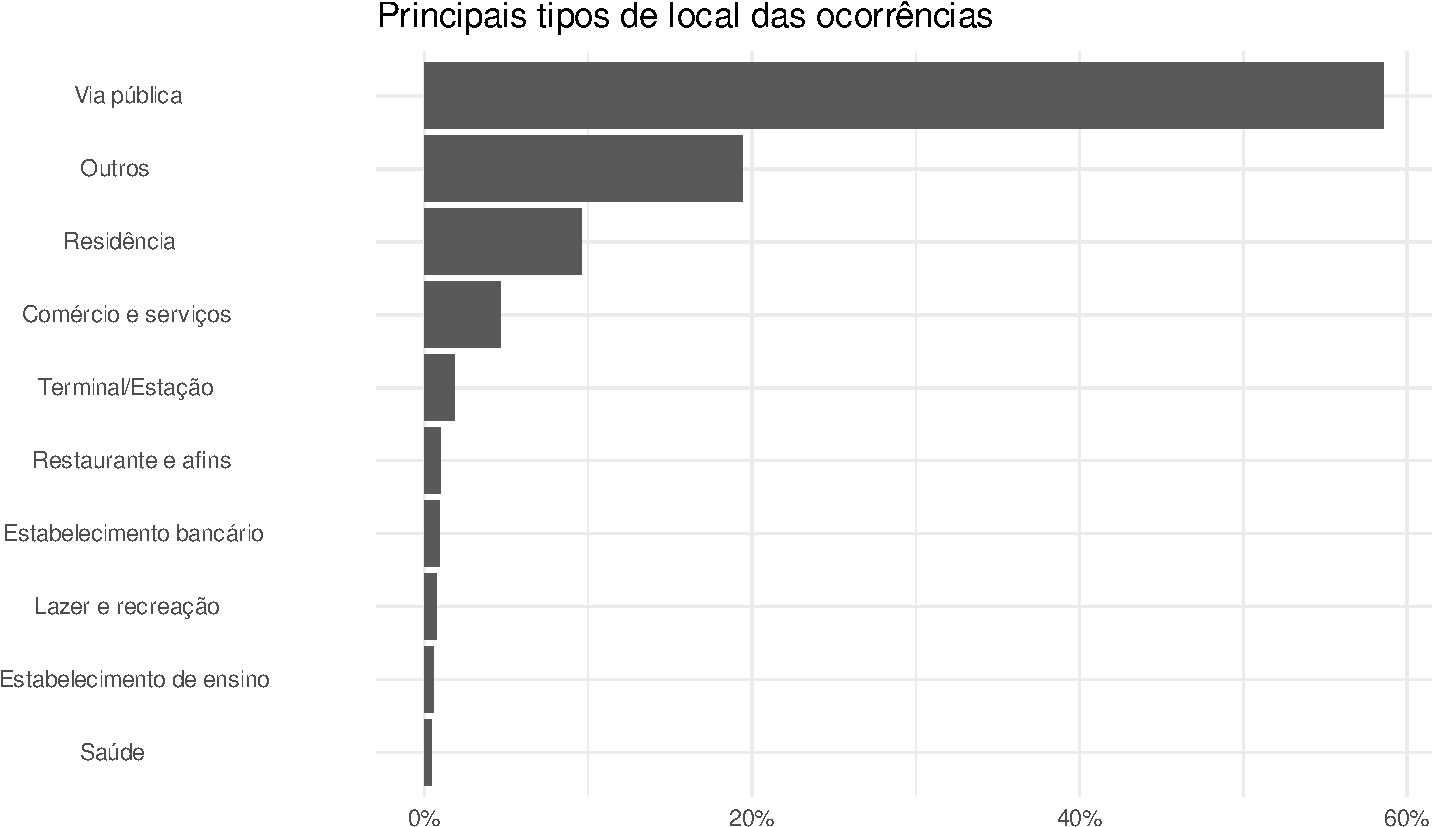
\includegraphics{relatorio_final_files/figure-latex/unnamed-chunk-7-1.pdf}

\hypertarget{localizauxe7uxe3o}{%
\subsection{Localização}\label{localizauxe7uxe3o}}

A seguir vemos como as ocorrências se distribuem geograficamente por São Paulo, com grande concentração na região central da cidade.

\begin{verbatim}
FALSE   |                                                                              |                                                                      |   0%  |                                                                              |======================================================================| 100%
FALSE Downloading: 770 B     Downloading: 770 B     Downloading: 1.2 kB     Downloading: 1.2 kB     Downloading: 1.7 kB     Downloading: 1.7 kB     Downloading: 1.7 kB     Downloading: 1.7 kB     Downloading: 1.8 kB     Downloading: 1.8 kB     Downloading: 1.9 kB     Downloading: 1.9 kB     Downloading: 1.9 kB     Downloading: 1.9 kB     Downloading: 1.9 kB     Downloading: 1.9 kB     Downloading: 2 kB     Downloading: 2 kB     Downloading: 2.1 kB     Downloading: 2.1 kB     Downloading: 2.1 kB     Downloading: 2.1 kB     Downloading: 2.1 kB     Downloading: 2.1 kB     Downloading: 2.1 kB     Downloading: 2.1 kB     Downloading: 2.1 kB     Downloading: 2.1 kB     Downloading: 4.5 kB     Downloading: 4.5 kB     Downloading: 4.5 kB     Downloading: 4.5 kB     Downloading: 4.5 kB     Downloading: 4.5 kB     Downloading: 13 kB     Downloading: 13 kB     Downloading: 13 kB     Downloading: 13 kB     Downloading: 13 kB     Downloading: 13 kB     Downloading: 21 kB     Downloading: 21 kB     Downloading: 21 kB     Downloading: 21 kB     Downloading: 21 kB     Downloading: 21 kB     Downloading: 21 kB     Downloading: 21 kB     Downloading: 29 kB     Downloading: 29 kB     Downloading: 29 kB     Downloading: 29 kB     Downloading: 29 kB     Downloading: 29 kB     Downloading: 37 kB     Downloading: 37 kB     Downloading: 37 kB     Downloading: 37 kB     Downloading: 37 kB     Downloading: 37 kB     Downloading: 37 kB     Downloading: 37 kB     Downloading: 45 kB     Downloading: 45 kB     Downloading: 45 kB     Downloading: 45 kB     Downloading: 45 kB     Downloading: 45 kB     Downloading: 53 kB     Downloading: 53 kB     Downloading: 53 kB     Downloading: 53 kB     Downloading: 53 kB     Downloading: 53 kB     Downloading: 53 kB     Downloading: 53 kB     Downloading: 61 kB     Downloading: 61 kB     Downloading: 61 kB     Downloading: 61 kB     Downloading: 61 kB     Downloading: 61 kB     Downloading: 61 kB     Downloading: 61 kB     Downloading: 61 kB     Downloading: 61 kB     Downloading: 69 kB     Downloading: 69 kB     Downloading: 69 kB     Downloading: 69 kB     Downloading: 69 kB     Downloading: 69 kB     Downloading: 69 kB     Downloading: 69 kB     Downloading: 77 kB     Downloading: 77 kB     Downloading: 77 kB     Downloading: 77 kB     Downloading: 77 kB     Downloading: 77 kB     Downloading: 77 kB     Downloading: 77 kB     Downloading: 85 kB     Downloading: 85 kB     Downloading: 85 kB     Downloading: 85 kB     Downloading: 85 kB     Downloading: 85 kB     Downloading: 85 kB     Downloading: 85 kB     Downloading: 94 kB     Downloading: 94 kB     Downloading: 94 kB     Downloading: 94 kB     Downloading: 94 kB     Downloading: 94 kB     Downloading: 94 kB     Downloading: 94 kB     Downloading: 94 kB     Downloading: 94 kB     Downloading: 100 kB     Downloading: 100 kB     Downloading: 100 kB     Downloading: 100 kB     Downloading: 100 kB     Downloading: 100 kB     Downloading: 100 kB     Downloading: 100 kB     Downloading: 100 kB     Downloading: 100 kB     Downloading: 110 kB     Downloading: 110 kB     Downloading: 110 kB     Downloading: 110 kB     Downloading: 110 kB     Downloading: 110 kB     Downloading: 110 kB     Downloading: 110 kB     Downloading: 110 kB     Downloading: 110 kB     Downloading: 120 kB     Downloading: 120 kB     Downloading: 120 kB     Downloading: 120 kB     Downloading: 120 kB     Downloading: 120 kB     Downloading: 120 kB     Downloading: 120 kB     Downloading: 130 kB     Downloading: 130 kB     Downloading: 130 kB     Downloading: 130 kB     Downloading: 130 kB     Downloading: 130 kB     Downloading: 130 kB     Downloading: 130 kB     Downloading: 130 kB     Downloading: 130 kB     Downloading: 130 kB     Downloading: 130 kB     Downloading: 130 kB     Downloading: 130 kB     Downloading: 130 kB     Downloading: 130 kB     Downloading: 130 kB     Downloading: 130 kB     Downloading: 140 kB     Downloading: 140 kB     Downloading: 140 kB     Downloading: 140 kB     Downloading: 140 kB     Downloading: 140 kB     Downloading: 150 kB     Downloading: 150 kB     Downloading: 150 kB     Downloading: 150 kB     Downloading: 150 kB     Downloading: 150 kB     Downloading: 150 kB     Downloading: 150 kB     Downloading: 160 kB     Downloading: 160 kB     Downloading: 160 kB     Downloading: 160 kB     Downloading: 160 kB     Downloading: 160 kB     Downloading: 160 kB     Downloading: 160 kB     Downloading: 160 kB     Downloading: 160 kB     Downloading: 160 kB     Downloading: 160 kB     Downloading: 170 kB     Downloading: 170 kB     Downloading: 170 kB     Downloading: 170 kB     Downloading: 170 kB     Downloading: 170 kB     Downloading: 170 kB     Downloading: 170 kB     Downloading: 170 kB     Downloading: 170 kB     Downloading: 170 kB     Downloading: 170 kB     Downloading: 170 kB     Downloading: 170 kB     Downloading: 170 kB     Downloading: 170 kB     Downloading: 180 kB     Downloading: 180 kB     Downloading: 180 kB     Downloading: 180 kB     Downloading: 180 kB     Downloading: 180 kB     Downloading: 180 kB     Downloading: 180 kB     Downloading: 190 kB     Downloading: 190 kB     Downloading: 190 kB     Downloading: 190 kB     Downloading: 190 kB     Downloading: 190 kB     Downloading: 190 kB     Downloading: 190 kB     Downloading: 190 kB     Downloading: 190 kB     Downloading: 190 kB     Downloading: 190 kB     Downloading: 200 kB     Downloading: 200 kB     Downloading: 200 kB     Downloading: 200 kB     Downloading: 200 kB     Downloading: 200 kB     Downloading: 210 kB     Downloading: 210 kB     Downloading: 210 kB     Downloading: 210 kB     Downloading: 210 kB     Downloading: 210 kB     Downloading: 210 kB     Downloading: 210 kB     Downloading: 210 kB     Downloading: 210 kB     Downloading: 210 kB     Downloading: 210 kB     Downloading: 210 kB     Downloading: 210 kB     Downloading: 210 kB     Downloading: 210 kB     Downloading: 210 kB     Downloading: 210 kB     Downloading: 210 kB     Downloading: 210 kB     Downloading: 220 kB     Downloading: 220 kB     Downloading: 220 kB     Downloading: 220 kB     Downloading: 220 kB     Downloading: 220 kB     Downloading: 220 kB     Downloading: 220 kB     Downloading: 220 kB     Downloading: 220 kB     Downloading: 230 kB     Downloading: 230 kB     Downloading: 230 kB     Downloading: 230 kB     Downloading: 230 kB     Downloading: 230 kB     Downloading: 240 kB     Downloading: 240 kB     Downloading: 240 kB     Downloading: 240 kB     Downloading: 240 kB     Downloading: 240 kB     Downloading: 240 kB     Downloading: 240 kB     Downloading: 250 kB     Downloading: 250 kB     Downloading: 250 kB     Downloading: 250 kB     Downloading: 250 kB     Downloading: 250 kB     Downloading: 250 kB     Downloading: 250 kB     Downloading: 250 kB     Downloading: 250 kB     Downloading: 260 kB     Downloading: 260 kB     Downloading: 260 kB     Downloading: 260 kB     Downloading: 260 kB     Downloading: 260 kB     Downloading: 260 kB     Downloading: 260 kB     Downloading: 260 kB     Downloading: 260 kB     Downloading: 260 kB     Downloading: 260 kB     Downloading: 260 kB     Downloading: 260 kB     Downloading: 260 kB     Downloading: 260 kB     Downloading: 260 kB     Downloading: 260 kB     Downloading: 270 kB     Downloading: 270 kB     Downloading: 270 kB     Downloading: 270 kB     Downloading: 270 kB     Downloading: 270 kB     Downloading: 280 kB     Downloading: 280 kB     Downloading: 280 kB     Downloading: 280 kB     Downloading: 280 kB     Downloading: 280 kB     Downloading: 280 kB     Downloading: 280 kB     Downloading: 290 kB     Downloading: 290 kB     Downloading: 290 kB     Downloading: 290 kB     Downloading: 290 kB     Downloading: 290 kB     Downloading: 290 kB     Downloading: 290 kB     Downloading: 290 kB     Downloading: 290 kB     Downloading: 290 kB     Downloading: 290 kB     Downloading: 300 kB     Downloading: 300 kB     Downloading: 300 kB     Downloading: 300 kB     Downloading: 300 kB     Downloading: 300 kB     Downloading: 300 kB     Downloading: 300 kB     Downloading: 300 kB     Downloading: 300 kB     Downloading: 300 kB     Downloading: 300 kB     Downloading: 300 kB     Downloading: 300 kB     Downloading: 300 kB     Downloading: 300 kB     Downloading: 310 kB     Downloading: 310 kB     Downloading: 310 kB     Downloading: 310 kB     Downloading: 310 kB     Downloading: 310 kB     Downloading: 310 kB     Downloading: 310 kB     Downloading: 310 kB     Downloading: 310 kB     Downloading: 320 kB     Downloading: 320 kB     Downloading: 320 kB     Downloading: 320 kB     Downloading: 320 kB     Downloading: 320 kB     Downloading: 330 kB     Downloading: 330 kB     Downloading: 330 kB     Downloading: 330 kB     Downloading: 330 kB     Downloading: 330 kB     Downloading: 330 kB     Downloading: 330 kB     Downloading: 340 kB     Downloading: 340 kB     Downloading: 340 kB     Downloading: 340 kB     Downloading: 340 kB     Downloading: 340 kB     Downloading: 340 kB     Downloading: 340 kB     Downloading: 340 kB     Downloading: 340 kB     Downloading: 340 kB     Downloading: 340 kB     Downloading: 340 kB     Downloading: 340 kB     Downloading: 340 kB     Downloading: 340 kB     Downloading: 350 kB     Downloading: 350 kB     Downloading: 350 kB     Downloading: 350 kB     Downloading: 350 kB     Downloading: 350 kB     Downloading: 350 kB     Downloading: 350 kB     Downloading: 360 kB     Downloading: 360 kB     Downloading: 360 kB     Downloading: 360 kB     Downloading: 360 kB     Downloading: 360 kB     Downloading: 360 kB     Downloading: 360 kB     Downloading: 370 kB     Downloading: 370 kB     Downloading: 370 kB     Downloading: 370 kB     Downloading: 370 kB     Downloading: 370 kB     Downloading: 370 kB     Downloading: 370 kB     Downloading: 380 kB     Downloading: 380 kB     Downloading: 380 kB     Downloading: 380 kB     Downloading: 380 kB     Downloading: 380 kB     Downloading: 380 kB     Downloading: 380 kB     Downloading: 380 kB     Downloading: 380 kB     Downloading: 380 kB     Downloading: 380 kB     Downloading: 380 kB     Downloading: 380 kB     Downloading: 390 kB     Downloading: 390 kB     Downloading: 390 kB     Downloading: 390 kB     Downloading: 390 kB     Downloading: 390 kB     Downloading: 400 kB     Downloading: 400 kB     Downloading: 400 kB     Downloading: 400 kB     Downloading: 400 kB     Downloading: 400 kB     Downloading: 400 kB     Downloading: 400 kB     Downloading: 400 kB     Downloading: 400 kB     Downloading: 410 kB     Downloading: 410 kB     Downloading: 410 kB     Downloading: 410 kB     Downloading: 410 kB     Downloading: 410 kB     Downloading: 420 kB     Downloading: 420 kB     Downloading: 420 kB     Downloading: 420 kB     Downloading: 420 kB     Downloading: 420 kB     Downloading: 420 kB     Downloading: 420 kB     Downloading: 430 kB     Downloading: 430 kB     Downloading: 430 kB     Downloading: 430 kB     Downloading: 430 kB     Downloading: 430 kB     Downloading: 430 kB     Downloading: 430 kB     Downloading: 430 kB     Downloading: 430 kB     Downloading: 430 kB     Downloading: 430 kB     Downloading: 430 kB     Downloading: 430 kB     Downloading: 430 kB     Downloading: 430 kB     Downloading: 440 kB     Downloading: 440 kB     Downloading: 440 kB     Downloading: 440 kB     Downloading: 440 kB     Downloading: 440 kB     Downloading: 440 kB     Downloading: 440 kB     Downloading: 440 kB     Downloading: 440 kB     Downloading: 450 kB     Downloading: 450 kB     Downloading: 450 kB     Downloading: 450 kB     Downloading: 450 kB     Downloading: 450 kB     Downloading: 450 kB     Downloading: 450 kB     Downloading: 450 kB     Downloading: 450 kB     Downloading: 460 kB     Downloading: 460 kB     Downloading: 460 kB     Downloading: 460 kB     Downloading: 460 kB     Downloading: 460 kB     Downloading: 470 kB     Downloading: 470 kB     Downloading: 470 kB     Downloading: 470 kB     Downloading: 470 kB     Downloading: 470 kB     Downloading: 470 kB     Downloading: 470 kB     Downloading: 470 kB     Downloading: 470 kB     Downloading: 470 kB     Downloading: 470 kB     Downloading: 470 kB     Downloading: 470 kB     Downloading: 470 kB     Downloading: 470 kB     Downloading: 480 kB     Downloading: 480 kB     Downloading: 480 kB     Downloading: 480 kB     Downloading: 480 kB     Downloading: 480 kB     Downloading: 490 kB     Downloading: 490 kB     Downloading: 490 kB     Downloading: 490 kB     Downloading: 490 kB     Downloading: 490 kB     Downloading: 490 kB     Downloading: 490 kB     Downloading: 490 kB     Downloading: 490 kB     Downloading: 500 kB     Downloading: 500 kB     Downloading: 500 kB     Downloading: 500 kB     Downloading: 500 kB     Downloading: 500 kB     Downloading: 510 kB     Downloading: 510 kB     Downloading: 510 kB     Downloading: 510 kB     Downloading: 510 kB     Downloading: 510 kB     Downloading: 510 kB     Downloading: 510 kB     Downloading: 510 kB     Downloading: 510 kB     Downloading: 510 kB     Downloading: 510 kB     Downloading: 520 kB     Downloading: 520 kB     Downloading: 520 kB     Downloading: 520 kB     Downloading: 520 kB     Downloading: 520 kB     Downloading: 530 kB     Downloading: 530 kB     Downloading: 530 kB     Downloading: 530 kB     Downloading: 530 kB     Downloading: 530 kB     Downloading: 530 kB     Downloading: 530 kB     Downloading: 530 kB     Downloading: 530 kB     Downloading: 540 kB     Downloading: 540 kB     Downloading: 540 kB     Downloading: 540 kB     Downloading: 540 kB     Downloading: 540 kB     Downloading: 540 kB     Downloading: 540 kB     Downloading: 540 kB     Downloading: 540 kB     Downloading: 540 kB     Downloading: 540 kB     Downloading: 550 kB     Downloading: 550 kB     Downloading: 550 kB     Downloading: 550 kB     Downloading: 550 kB     Downloading: 550 kB     Downloading: 550 kB     Downloading: 550 kB     Downloading: 550 kB     Downloading: 550 kB     Downloading: 550 kB     Downloading: 550 kB     Downloading: 550 kB     Downloading: 550 kB     Downloading: 550 kB     Downloading: 550 kB     Downloading: 550 kB     Downloading: 550 kB     Downloading: 560 kB     Downloading: 560 kB     Downloading: 560 kB     Downloading: 560 kB     Downloading: 560 kB     Downloading: 560 kB     Downloading: 570 kB     Downloading: 570 kB     Downloading: 570 kB     Downloading: 570 kB     Downloading: 570 kB     Downloading: 570 kB     Downloading: 570 kB     Downloading: 570 kB     Downloading: 580 kB     Downloading: 580 kB     Downloading: 580 kB     Downloading: 580 kB     Downloading: 580 kB     Downloading: 580 kB     Downloading: 590 kB     Downloading: 590 kB     Downloading: 590 kB     Downloading: 590 kB     Downloading: 590 kB     Downloading: 590 kB     Downloading: 600 kB     Downloading: 600 kB     Downloading: 600 kB     Downloading: 600 kB     Downloading: 600 kB     Downloading: 600 kB     Downloading: 600 kB     Downloading: 600 kB     Downloading: 600 kB     Downloading: 600 kB     Downloading: 600 kB     Downloading: 600 kB     Downloading: 600 kB     Downloading: 600 kB     Downloading: 600 kB     Downloading: 600 kB     Downloading: 610 kB     Downloading: 610 kB     Downloading: 610 kB     Downloading: 610 kB     Downloading: 610 kB     Downloading: 610 kB     Downloading: 620 kB     Downloading: 620 kB     Downloading: 620 kB     Downloading: 620 kB     Downloading: 620 kB     Downloading: 620 kB     Downloading: 620 kB     Downloading: 620 kB     Downloading: 620 kB     Downloading: 620 kB     Downloading: 630 kB     Downloading: 630 kB     Downloading: 630 kB     Downloading: 630 kB     Downloading: 630 kB     Downloading: 630 kB     Downloading: 630 kB     Downloading: 630 kB     Downloading: 640 kB     Downloading: 640 kB     Downloading: 640 kB     Downloading: 640 kB     Downloading: 640 kB     Downloading: 640 kB     Downloading: 640 kB     Downloading: 640 kB     Downloading: 640 kB     Downloading: 640 kB     Downloading: 640 kB     Downloading: 640 kB     Downloading: 650 kB     Downloading: 650 kB     Downloading: 650 kB     Downloading: 650 kB     Downloading: 650 kB     Downloading: 650 kB     Downloading: 660 kB     Downloading: 660 kB     Downloading: 660 kB     Downloading: 660 kB     Downloading: 660 kB     Downloading: 660 kB     Downloading: 660 kB     Downloading: 660 kB     Downloading: 660 kB     Downloading: 660 kB     Downloading: 670 kB     Downloading: 670 kB     Downloading: 670 kB     Downloading: 670 kB     Downloading: 670 kB     Downloading: 670 kB     Downloading: 670 kB     Downloading: 670 kB     Downloading: 670 kB     Downloading: 670 kB     Downloading: 680 kB     Downloading: 680 kB     Downloading: 680 kB     Downloading: 680 kB     Downloading: 680 kB     Downloading: 680 kB     Downloading: 680 kB     Downloading: 680 kB     Downloading: 680 kB     Downloading: 680 kB     Downloading: 680 kB     Downloading: 680 kB     Downloading: 680 kB     Downloading: 680 kB     Downloading: 680 kB     Downloading: 680 kB     Downloading: 690 kB     Downloading: 690 kB     Downloading: 690 kB     Downloading: 690 kB     Downloading: 690 kB     Downloading: 690 kB     Downloading: 700 kB     Downloading: 700 kB     Downloading: 700 kB     Downloading: 700 kB     Downloading: 700 kB     Downloading: 700 kB     Downloading: 700 kB     Downloading: 700 kB     Downloading: 700 kB     Downloading: 700 kB     Downloading: 700 kB     Downloading: 700 kB     Downloading: 710 kB     Downloading: 710 kB     Downloading: 710 kB     Downloading: 710 kB     Downloading: 710 kB     Downloading: 710 kB     Downloading: 720 kB     Downloading: 720 kB     Downloading: 720 kB     Downloading: 720 kB     Downloading: 720 kB     Downloading: 720 kB     Downloading: 720 kB     Downloading: 720 kB     Downloading: 720 kB     Downloading: 720 kB     Downloading: 720 kB     Downloading: 720 kB     Downloading: 720 kB     Downloading: 720 kB     Downloading: 730 kB     Downloading: 730 kB     Downloading: 730 kB     Downloading: 730 kB     Downloading: 730 kB     Downloading: 730 kB     Downloading: 730 kB     Downloading: 730 kB     Downloading: 730 kB     Downloading: 730 kB     Downloading: 730 kB     Downloading: 730 kB     Downloading: 730 kB     Downloading: 730 kB     Downloading: 730 kB     Downloading: 730 kB     Downloading: 730 kB     Downloading: 730 kB     Downloading: 730 kB     Downloading: 730 kB     Downloading: 740 kB     Downloading: 740 kB     Downloading: 740 kB     Downloading: 740 kB     Downloading: 740 kB     Downloading: 740 kB     Downloading: 750 kB     Downloading: 750 kB     Downloading: 750 kB     Downloading: 750 kB     Downloading: 750 kB     Downloading: 750 kB     Downloading: 760 kB     Downloading: 760 kB     Downloading: 760 kB     Downloading: 760 kB     Downloading: 760 kB     Downloading: 760 kB     Downloading: 760 kB     Downloading: 760 kB     Downloading: 760 kB     Downloading: 760 kB     Downloading: 770 kB     Downloading: 770 kB     Downloading: 770 kB     Downloading: 770 kB     Downloading: 770 kB     Downloading: 770 kB     Downloading: 770 kB     Downloading: 770 kB     Downloading: 770 kB     Downloading: 770 kB     Downloading: 770 kB     Downloading: 770 kB     Downloading: 780 kB     Downloading: 780 kB     Downloading: 780 kB     Downloading: 780 kB     Downloading: 780 kB     Downloading: 780 kB     Downloading: 780 kB     Downloading: 780 kB     Downloading: 780 kB     Downloading: 780 kB     Downloading: 780 kB     Downloading: 780 kB     Downloading: 780 kB     Downloading: 780 kB     Downloading: 790 kB     Downloading: 790 kB     Downloading: 790 kB     Downloading: 790 kB     Downloading: 790 kB     Downloading: 790 kB     Downloading: 790 kB     Downloading: 790 kB     Downloading: 790 kB     Downloading: 790 kB     Downloading: 790 kB     Downloading: 790 kB     Downloading: 800 kB     Downloading: 800 kB     Downloading: 800 kB     Downloading: 800 kB     Downloading: 800 kB     Downloading: 800 kB     Downloading: 800 kB     Downloading: 800 kB     Downloading: 800 kB     Downloading: 800 kB     Downloading: 800 kB     Downloading: 800 kB     Downloading: 800 kB     Downloading: 800 kB     Downloading: 810 kB     Downloading: 810 kB     Downloading: 810 kB     Downloading: 810 kB     Downloading: 810 kB     Downloading: 810 kB     Downloading: 810 kB     Downloading: 810 kB     Downloading: 810 kB     Downloading: 810 kB     Downloading: 810 kB     Downloading: 810 kB     Downloading: 820 kB     Downloading: 820 kB     Downloading: 820 kB     Downloading: 820 kB     Downloading: 820 kB     Downloading: 820 kB     Downloading: 830 kB     Downloading: 830 kB     Downloading: 830 kB     Downloading: 830 kB     Downloading: 830 kB     Downloading: 830 kB     Downloading: 840 kB     Downloading: 840 kB     Downloading: 840 kB     Downloading: 840 kB     Downloading: 840 kB     Downloading: 840 kB     Downloading: 850 kB     Downloading: 850 kB     Downloading: 850 kB     Downloading: 850 kB     Downloading: 850 kB     Downloading: 850 kB     Downloading: 850 kB     Downloading: 850 kB     Downloading: 850 kB     Downloading: 850 kB     Downloading: 850 kB     Downloading: 850 kB     Downloading: 850 kB     Downloading: 850 kB     Downloading: 860 kB     Downloading: 860 kB     Downloading: 860 kB     Downloading: 860 kB     Downloading: 860 kB     Downloading: 860 kB     Downloading: 870 kB     Downloading: 870 kB     Downloading: 870 kB     Downloading: 870 kB     Downloading: 870 kB     Downloading: 870 kB     Downloading: 880 kB     Downloading: 880 kB     Downloading: 880 kB     Downloading: 880 kB     Downloading: 880 kB     Downloading: 880 kB     Downloading: 890 kB     Downloading: 890 kB     Downloading: 890 kB     Downloading: 890 kB     Downloading: 890 kB     Downloading: 890 kB     Downloading: 900 kB     Downloading: 900 kB     Downloading: 900 kB     Downloading: 900 kB     Downloading: 900 kB     Downloading: 900 kB     Downloading: 900 kB     Downloading: 900 kB     Downloading: 900 kB     Downloading: 900 kB     Downloading: 900 kB     Downloading: 900 kB     Downloading: 900 kB     Downloading: 900 kB     Downloading: 900 kB     Downloading: 900 kB     Downloading: 900 kB     Downloading: 900 kB     Downloading: 910 kB     Downloading: 910 kB     Downloading: 910 kB     Downloading: 910 kB     Downloading: 910 kB     Downloading: 910 kB     Downloading: 920 kB     Downloading: 920 kB     Downloading: 920 kB     Downloading: 920 kB     Downloading: 920 kB     Downloading: 920 kB     Downloading: 930 kB     Downloading: 930 kB     Downloading: 930 kB     Downloading: 930 kB     Downloading: 930 kB     Downloading: 930 kB     Downloading: 940 kB     Downloading: 940 kB     Downloading: 940 kB     Downloading: 940 kB     Downloading: 940 kB     Downloading: 940 kB     Downloading: 940 kB     Downloading: 940 kB     Downloading: 940 kB     Downloading: 940 kB     Downloading: 940 kB     Downloading: 940 kB     Downloading: 950 kB     Downloading: 950 kB     Downloading: 950 kB     Downloading: 950 kB     Downloading: 950 kB     Downloading: 950 kB     Downloading: 960 kB     Downloading: 960 kB     Downloading: 960 kB     Downloading: 960 kB     Downloading: 960 kB     Downloading: 960 kB     Downloading: 970 kB     Downloading: 970 kB     Downloading: 970 kB     Downloading: 970 kB     Downloading: 970 kB     Downloading: 970 kB     Downloading: 980 kB     Downloading: 980 kB     Downloading: 980 kB     Downloading: 980 kB     Downloading: 980 kB     Downloading: 980 kB     Downloading: 980 kB     Downloading: 980 kB     Downloading: 980 kB     Downloading: 980 kB     Downloading: 980 kB     Downloading: 980 kB     Downloading: 980 kB     Downloading: 980 kB     Downloading: 980 kB     Downloading: 980 kB     Downloading: 990 kB     Downloading: 990 kB     Downloading: 990 kB     Downloading: 990 kB     Downloading: 990 kB     Downloading: 990 kB     Downloading: 1 MB     Downloading: 1 MB     Downloading: 1 MB     Downloading: 1 MB     Downloading: 1 MB     Downloading: 1 MB     Downloading: 1 MB     Downloading: 1 MB     Downloading: 1 MB     Downloading: 1 MB     Downloading: 1 MB     Downloading: 1 MB     Downloading: 1 MB     Downloading: 1 MB     Downloading: 1 MB     Downloading: 1 MB     Downloading: 1 MB     Downloading: 1 MB     Downloading: 1 MB     Downloading: 1 MB     Downloading: 1 MB     Downloading: 1 MB     Downloading: 1 MB     Downloading: 1 MB     Downloading: 1 MB     Downloading: 1 MB     Downloading: 1 MB     Downloading: 1 MB     Downloading: 1 MB     Downloading: 1 MB     Downloading: 1 MB     Downloading: 1 MB     Downloading: 1 MB     Downloading: 1 MB     Downloading: 1 MB     Downloading: 1 MB     Downloading: 1 MB     Downloading: 1 MB     Downloading: 1 MB     Downloading: 1 MB     Downloading: 1 MB     Downloading: 1 MB     Downloading: 1 MB     Downloading: 1 MB     Downloading: 1 MB     Downloading: 1 MB     Downloading: 1 MB     Downloading: 1 MB     Downloading: 1 MB     Downloading: 1 MB     Downloading: 1 MB     Downloading: 1 MB     Downloading: 1 MB     Downloading: 1 MB     Downloading: 1 MB     Downloading: 1 MB     Downloading: 1 MB     Downloading: 1 MB     Downloading: 1.1 MB     Downloading: 1.1 MB     Downloading: 1.1 MB     Downloading: 1.1 MB     Downloading: 1.1 MB     Downloading: 1.1 MB     Downloading: 1.1 MB     Downloading: 1.1 MB     Downloading: 1.1 MB     Downloading: 1.1 MB     Downloading: 1.1 MB     Downloading: 1.1 MB     Downloading: 1.1 MB     Downloading: 1.1 MB     Downloading: 1.1 MB     Downloading: 1.1 MB     Downloading: 1.1 MB     Downloading: 1.1 MB     Downloading: 1.1 MB     Downloading: 1.1 MB     Downloading: 1.1 MB     Downloading: 1.1 MB     Downloading: 1.1 MB     Downloading: 1.1 MB     Downloading: 1.1 MB     Downloading: 1.1 MB     Downloading: 1.1 MB     Downloading: 1.1 MB     Downloading: 1.1 MB     Downloading: 1.1 MB     Downloading: 1.1 MB     Downloading: 1.1 MB     Downloading: 1.1 MB     Downloading: 1.1 MB     Downloading: 1.1 MB     Downloading: 1.1 MB     Downloading: 1.1 MB     Downloading: 1.1 MB     Downloading: 1.1 MB     Downloading: 1.1 MB     Downloading: 1.1 MB     Downloading: 1.1 MB     Downloading: 1.1 MB     Downloading: 1.1 MB     Downloading: 1.1 MB     Downloading: 1.1 MB     Downloading: 1.1 MB     Downloading: 1.1 MB     Downloading: 1.1 MB     Downloading: 1.1 MB     Downloading: 1.1 MB     Downloading: 1.1 MB     Downloading: 1.1 MB     Downloading: 1.1 MB     Downloading: 1.1 MB     Downloading: 1.1 MB     Downloading: 1.1 MB     Downloading: 1.1 MB     Downloading: 1.1 MB     Downloading: 1.1 MB     Downloading: 1.1 MB     Downloading: 1.1 MB     Downloading: 1.1 MB     Downloading: 1.1 MB     Downloading: 1.1 MB     Downloading: 1.1 MB     Downloading: 1.1 MB     Downloading: 1.1 MB     Downloading: 1.1 MB     Downloading: 1.1 MB     Downloading: 1.1 MB     Downloading: 1.1 MB     Downloading: 1.1 MB     Downloading: 1.1 MB     Downloading: 1.1 MB     Downloading: 1.1 MB     Downloading: 1.1 MB     Downloading: 1.1 MB     Downloading: 1.1 MB     Downloading: 1.1 MB     Downloading: 1.1 MB     Downloading: 1.1 MB     Downloading: 1.1 MB     Downloading: 1.1 MB     Downloading: 1.1 MB     Downloading: 1.1 MB     Downloading: 1.1 MB     Downloading: 1.1 MB     Downloading: 1.1 MB     Downloading: 1.1 MB     Downloading: 1.1 MB     Downloading: 1.1 MB     Downloading: 1.1 MB     Downloading: 1.1 MB     Downloading: 1.2 MB     Downloading: 1.2 MB     Downloading: 1.2 MB     Downloading: 1.2 MB     Downloading: 1.2 MB     Downloading: 1.2 MB     Downloading: 1.2 MB     Downloading: 1.2 MB     Downloading: 1.2 MB     Downloading: 1.2 MB     Downloading: 1.2 MB     Downloading: 1.2 MB     Downloading: 1.2 MB     Downloading: 1.2 MB     Downloading: 1.2 MB     Downloading: 1.2 MB     Downloading: 1.2 MB     Downloading: 1.2 MB     Downloading: 1.2 MB     Downloading: 1.2 MB     Downloading: 1.2 MB     Downloading: 1.2 MB     Downloading: 1.2 MB     Downloading: 1.2 MB     Downloading: 1.2 MB     Downloading: 1.2 MB     Downloading: 1.2 MB     Downloading: 1.2 MB     Downloading: 1.2 MB     Downloading: 1.2 MB     Downloading: 1.2 MB     Downloading: 1.2 MB     Downloading: 1.2 MB     Downloading: 1.2 MB     Downloading: 1.2 MB     Downloading: 1.2 MB     Downloading: 1.2 MB     Downloading: 1.2 MB     Downloading: 1.2 MB     Downloading: 1.2 MB     Downloading: 1.2 MB     Downloading: 1.2 MB     Downloading: 1.2 MB     Downloading: 1.2 MB     Downloading: 1.2 MB     Downloading: 1.2 MB     Downloading: 1.2 MB     Downloading: 1.2 MB     Downloading: 1.2 MB     Downloading: 1.2 MB     Downloading: 1.2 MB     Downloading: 1.2 MB     Downloading: 1.2 MB     Downloading: 1.2 MB     Downloading: 1.2 MB     Downloading: 1.2 MB     Downloading: 1.2 MB     Downloading: 1.2 MB     Downloading: 1.2 MB     Downloading: 1.2 MB     Downloading: 1.2 MB     Downloading: 1.2 MB     Downloading: 1.2 MB     Downloading: 1.2 MB     Downloading: 1.2 MB     Downloading: 1.2 MB     Downloading: 1.2 MB     Downloading: 1.2 MB     Downloading: 1.2 MB     Downloading: 1.2 MB     Downloading: 1.2 MB     Downloading: 1.2 MB     Downloading: 1.2 MB     Downloading: 1.2 MB     Downloading: 1.2 MB     Downloading: 1.2 MB     Downloading: 1.2 MB     Downloading: 1.2 MB     Downloading: 1.2 MB     Downloading: 1.2 MB     Downloading: 1.3 MB     Downloading: 1.3 MB     Downloading: 1.3 MB     Downloading: 1.3 MB     Downloading: 1.3 MB     Downloading: 1.3 MB     Downloading: 1.3 MB     Downloading: 1.3 MB     Downloading: 1.3 MB     Downloading: 1.3 MB     Downloading: 1.3 MB     Downloading: 1.3 MB     Downloading: 1.3 MB     Downloading: 1.3 MB     Downloading: 1.3 MB     Downloading: 1.3 MB     Downloading: 1.3 MB     Downloading: 1.3 MB     Downloading: 1.3 MB     Downloading: 1.3 MB     Downloading: 1.3 MB     Downloading: 1.3 MB     Downloading: 1.3 MB     Downloading: 1.3 MB     Downloading: 1.3 MB     Downloading: 1.3 MB     Downloading: 1.3 MB     Downloading: 1.3 MB     Downloading: 1.3 MB     Downloading: 1.3 MB     Downloading: 1.3 MB     Downloading: 1.3 MB     Downloading: 1.3 MB     Downloading: 1.3 MB     Downloading: 1.3 MB     Downloading: 1.3 MB     Downloading: 1.3 MB     Downloading: 1.3 MB     Downloading: 1.3 MB     Downloading: 1.3 MB     Downloading: 1.3 MB     Downloading: 1.3 MB     Downloading: 1.3 MB     Downloading: 1.3 MB     Downloading: 1.3 MB     Downloading: 1.3 MB     Downloading: 1.3 MB     Downloading: 1.3 MB     Downloading: 1.3 MB     Downloading: 1.3 MB     Downloading: 1.3 MB     Downloading: 1.3 MB     Downloading: 1.3 MB     Downloading: 1.3 MB     Downloading: 1.3 MB     Downloading: 1.3 MB     Downloading: 1.3 MB     Downloading: 1.3 MB     Downloading: 1.3 MB     Downloading: 1.3 MB     Downloading: 1.3 MB     Downloading: 1.3 MB     Downloading: 1.3 MB     Downloading: 1.3 MB     Downloading: 1.3 MB     Downloading: 1.3 MB     Downloading: 1.3 MB     Downloading: 1.3 MB     Downloading: 1.3 MB     Downloading: 1.3 MB     Downloading: 1.3 MB     Downloading: 1.3 MB     Downloading: 1.3 MB     Downloading: 1.3 MB     Downloading: 1.3 MB     Downloading: 1.3 MB     Downloading: 1.3 MB     Downloading: 1.3 MB     Downloading: 1.3 MB     Downloading: 1.3 MB     Downloading: 1.3 MB     Downloading: 1.3 MB     Downloading: 1.3 MB     Downloading: 1.3 MB     Downloading: 1.3 MB     Downloading: 1.3 MB     Downloading: 1.3 MB     Downloading: 1.3 MB     Downloading: 1.3 MB     Downloading: 1.3 MB     Downloading: 1.3 MB     Downloading: 1.3 MB     Downloading: 1.3 MB     Downloading: 1.3 MB     Downloading: 1.3 MB     Downloading: 1.3 MB     Downloading: 1.3 MB     Downloading: 1.3 MB     Downloading: 1.3 MB     Downloading: 1.3 MB     Downloading: 1.3 MB     Downloading: 1.3 MB     Downloading: 1.3 MB     Downloading: 1.3 MB     Downloading: 1.3 MB     Downloading: 1.3 MB     Downloading: 1.3 MB     Downloading: 1.3 MB     Downloading: 1.3 MB     Downloading: 1.3 MB     Downloading: 1.3 MB     Downloading: 1.3 MB     Downloading: 1.3 MB     Downloading: 1.3 MB     Downloading: 1.3 MB     Downloading: 1.3 MB     Downloading: 1.3 MB     Downloading: 1.3 MB     Downloading: 1.4 MB     Downloading: 1.4 MB     Downloading: 1.4 MB     Downloading: 1.4 MB     Downloading: 1.4 MB     Downloading: 1.4 MB     Downloading: 1.4 MB     Downloading: 1.4 MB     Downloading: 1.4 MB     Downloading: 1.4 MB     Downloading: 1.4 MB     Downloading: 1.4 MB     Downloading: 1.4 MB     Downloading: 1.4 MB     Downloading: 1.4 MB     Downloading: 1.4 MB     Downloading: 1.4 MB     Downloading: 1.4 MB     Downloading: 1.4 MB     Downloading: 1.4 MB     Downloading: 1.4 MB     Downloading: 1.4 MB     Downloading: 1.4 MB     Downloading: 1.4 MB     Downloading: 1.4 MB     Downloading: 1.4 MB     Downloading: 1.4 MB     Downloading: 1.4 MB     Downloading: 1.4 MB     Downloading: 1.4 MB     Downloading: 1.4 MB     Downloading: 1.4 MB     Downloading: 1.4 MB     Downloading: 1.4 MB     Downloading: 1.4 MB     Downloading: 1.4 MB     Downloading: 1.4 MB     Downloading: 1.4 MB     Downloading: 1.4 MB     Downloading: 1.4 MB     Downloading: 1.4 MB     Downloading: 1.4 MB     Downloading: 1.4 MB     Downloading: 1.4 MB     Downloading: 1.4 MB     Downloading: 1.4 MB     Downloading: 1.4 MB     Downloading: 1.4 MB     Downloading: 1.4 MB     Downloading: 1.4 MB     Downloading: 1.4 MB     Downloading: 1.4 MB     Downloading: 1.4 MB     Downloading: 1.4 MB     Downloading: 1.4 MB     Downloading: 1.4 MB     Downloading: 1.4 MB     Downloading: 1.4 MB     Downloading: 1.4 MB     Downloading: 1.4 MB     Downloading: 1.4 MB     Downloading: 1.4 MB     Downloading: 1.4 MB     Downloading: 1.4 MB     Downloading: 1.4 MB     Downloading: 1.4 MB     Downloading: 1.4 MB     Downloading: 1.4 MB     Downloading: 1.4 MB     Downloading: 1.4 MB     Downloading: 1.4 MB     Downloading: 1.4 MB     Downloading: 1.4 MB     Downloading: 1.4 MB     Downloading: 1.4 MB     Downloading: 1.4 MB     Downloading: 1.4 MB     Downloading: 1.4 MB     Downloading: 1.4 MB     Downloading: 1.4 MB     Downloading: 1.4 MB     Downloading: 1.4 MB     Downloading: 1.4 MB     Downloading: 1.4 MB     Downloading: 1.4 MB     Downloading: 1.4 MB     Downloading: 1.4 MB     Downloading: 1.4 MB     Downloading: 1.4 MB     Downloading: 1.4 MB     Downloading: 1.4 MB     Downloading: 1.4 MB     Downloading: 1.4 MB     Downloading: 1.4 MB     Downloading: 1.4 MB     Downloading: 1.4 MB     Downloading: 1.4 MB     Downloading: 1.4 MB     Downloading: 1.4 MB     Downloading: 1.4 MB     Downloading: 1.4 MB     Downloading: 1.4 MB     Downloading: 1.4 MB     Downloading: 1.4 MB
\end{verbatim}

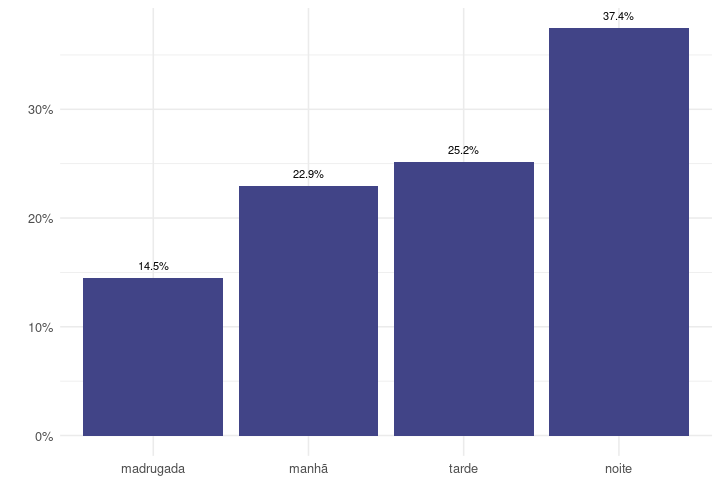
\includegraphics{relatorio_final_files/figure-latex/unnamed-chunk-8-1.pdf}

Considerando nossa amostra utilizada na modelagem, e vendo as categorias de período, chegamos ao seguinte mapa:

\begin{figure}
\centering
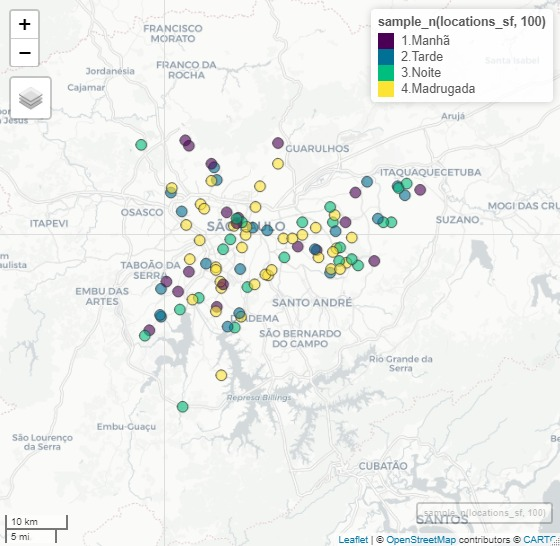
\includegraphics{assets/img/output_early_viz.jpeg}
\caption{Localização e período}
\end{figure}

\hypertarget{sexo-e-idade-das-vuxedtimas}{%
\subsection{Sexo e idade das vítimas}\label{sexo-e-idade-das-vuxedtimas}}

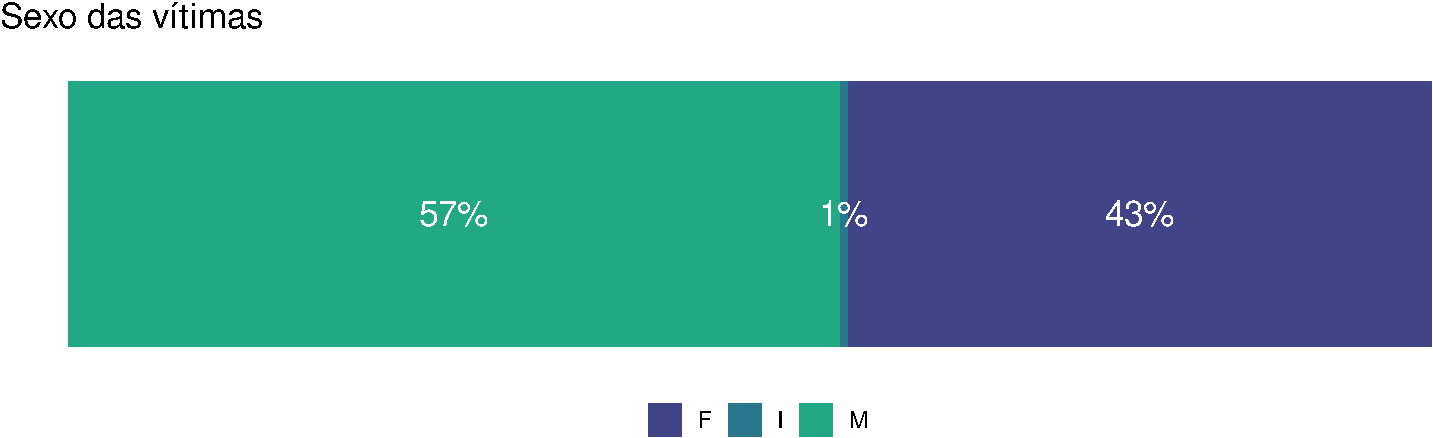
\includegraphics{relatorio_final_files/figure-latex/unnamed-chunk-9-1.pdf} 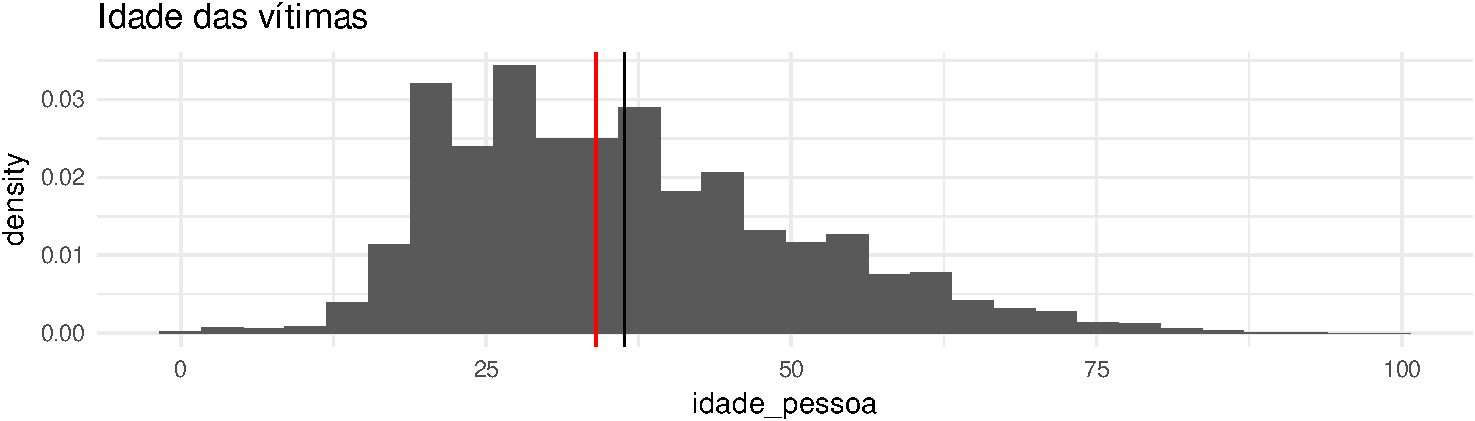
\includegraphics{relatorio_final_files/figure-latex/unnamed-chunk-9-2.pdf}

\hypertarget{tipificauxe7uxe3o}{%
\subsection{Tipificação}\label{tipificauxe7uxe3o}}

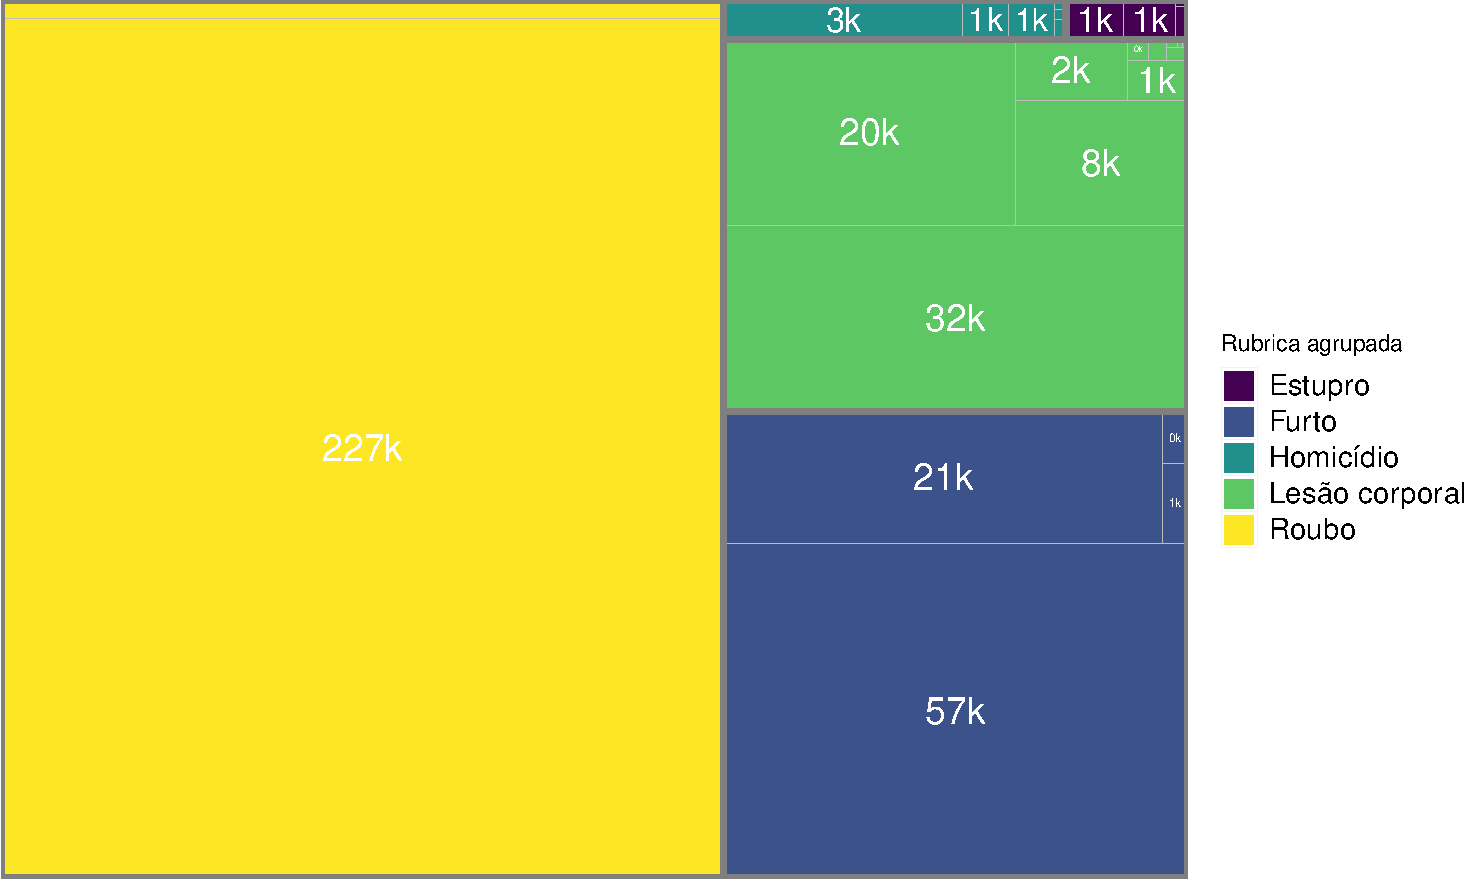
\includegraphics{relatorio_final_files/figure-latex/unnamed-chunk-10-1.pdf}

\hypertarget{distribuiuxe7uxe3o-da-idade-por-cor}{%
\subsection{Distribuição da idade por cor}\label{distribuiuxe7uxe3o-da-idade-por-cor}}

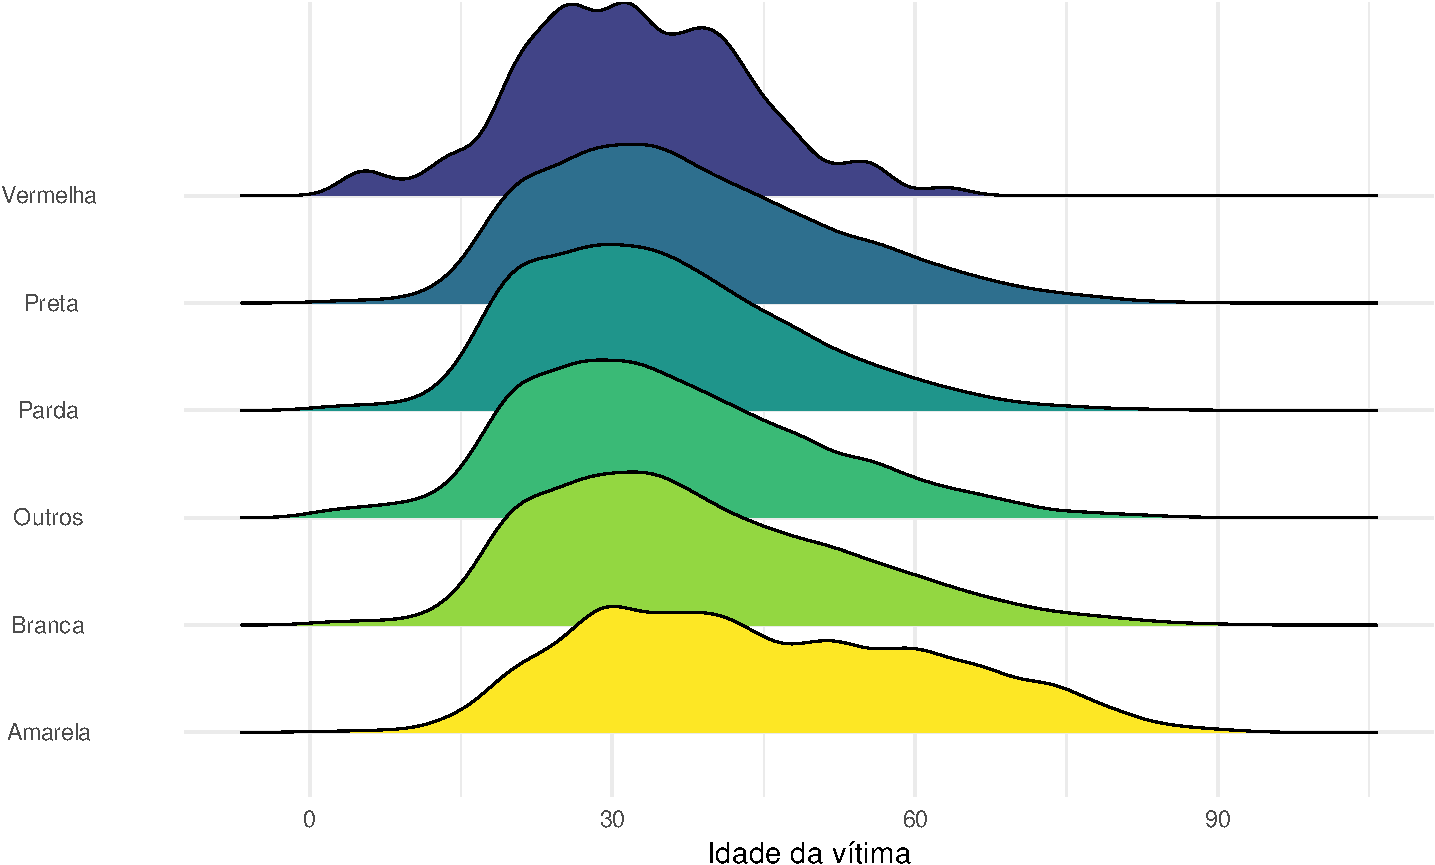
\includegraphics{relatorio_final_files/figure-latex/unnamed-chunk-11-1.pdf}

\hypertarget{vuxedtimas-fatais}{%
\subsection{Vítimas fatais}\label{vuxedtimas-fatais}}

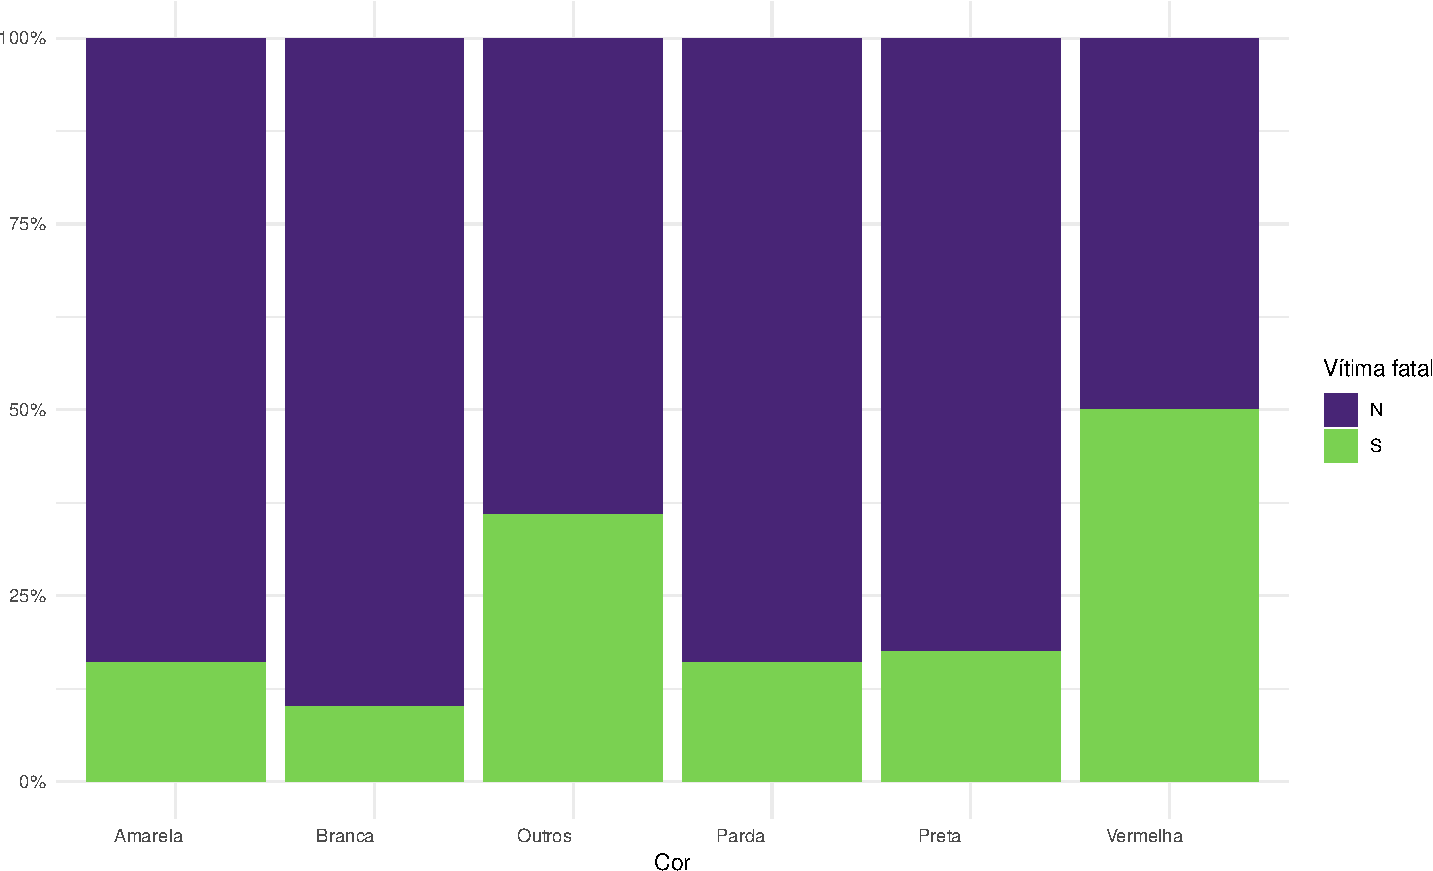
\includegraphics{relatorio_final_files/figure-latex/unnamed-chunk-12-1.pdf}

\hypertarget{horuxe1rio-e-dia-da-semana}{%
\subsection{Horário e dia da semana}\label{horuxe1rio-e-dia-da-semana}}

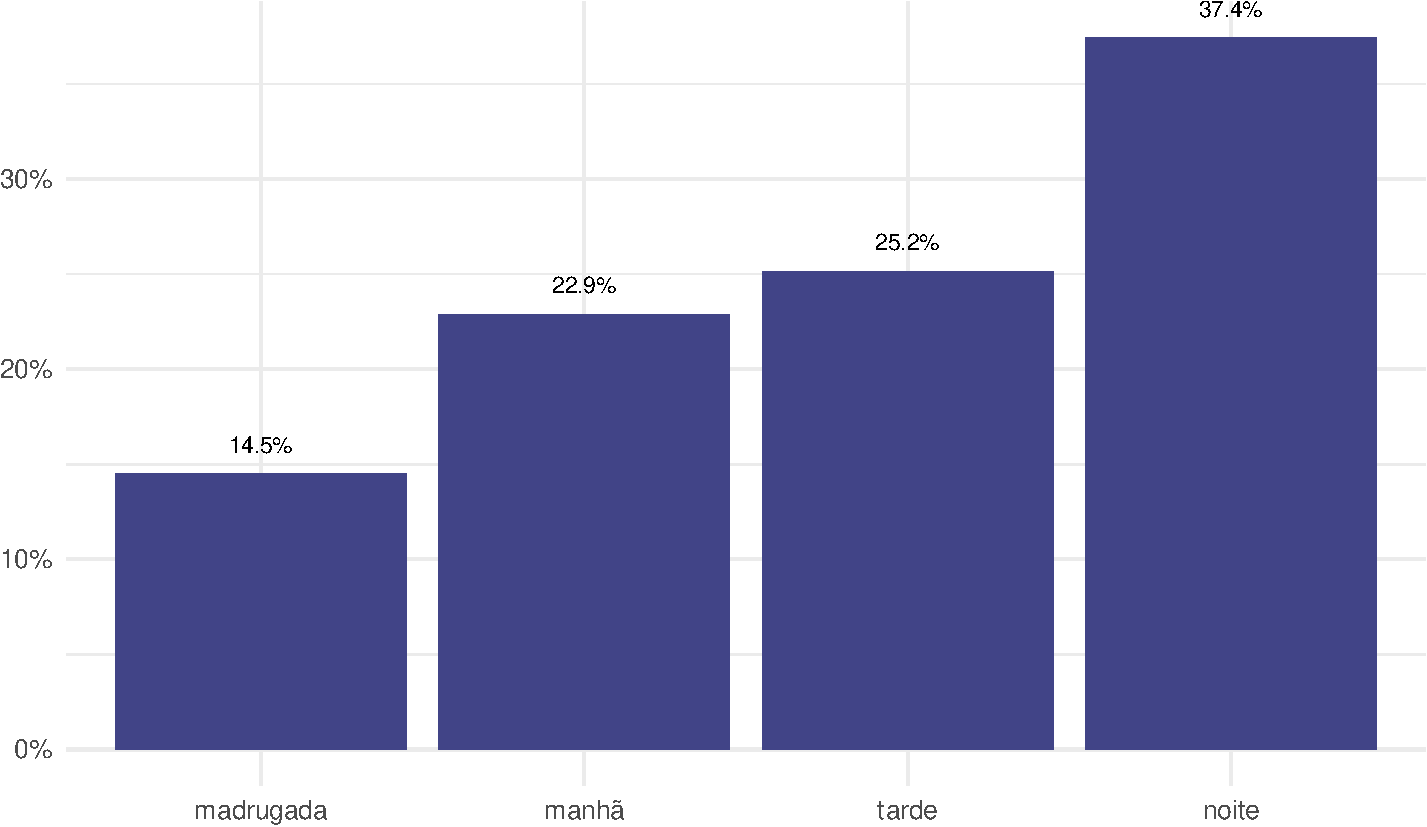
\includegraphics{relatorio_final_files/figure-latex/unnamed-chunk-13-1.pdf}

\hypertarget{random-forest-1}{%
\section{Random Forest}\label{random-forest-1}}

Avaliando os métodos, e começando com a Random Forest, vemos que a acurácia está em torno de 36\%, tanto na base de desenvolvimento quanto de teste. O parâmetro de mínimo de observações por folha definido em 20 contribui para que não haja overfitting no ajuste do modelo. Além da acurácia, as curvas ROC indicam que o acerto não é tão diferente entre as classes, e as proporções da saída do modelo estão em equilíbrio.

\begin{verbatim}
FALSE # A tibble: 2 x 3
FALSE   .metric  .estimator .estimate
FALSE   <chr>    <chr>          <dbl>
FALSE 1 accuracy multiclass     0.371
FALSE 2 kap      multiclass     0.161
\end{verbatim}

\begin{verbatim}
FALSE # A tibble: 2 x 3
FALSE   .metric  .estimator .estimate
FALSE   <chr>    <chr>          <dbl>
FALSE 1 accuracy multiclass     0.365
FALSE 2 kap      multiclass     0.144
\end{verbatim}

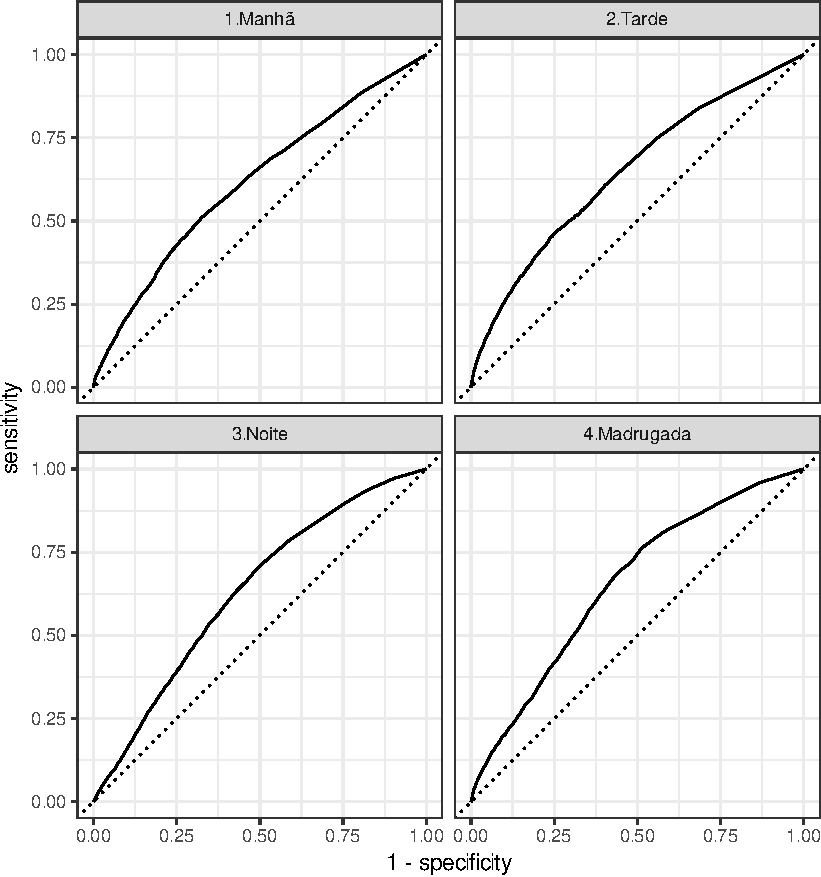
\includegraphics{relatorio_final_files/figure-latex/item Rforest-1.pdf}

\begin{verbatim}
FALSE .
FALSE 4.Madrugada     1.Manhã     2.Tarde     3.Noite 
FALSE  0.30220000  0.07806667  0.28940000  0.33033333
\end{verbatim}

A imagem abaixo traz uma representação gráfica da proporção de acertos e erros em uma amostra selecionada, levando em conta a distribuição espacial dos dados.

\begin{figure}
\centering
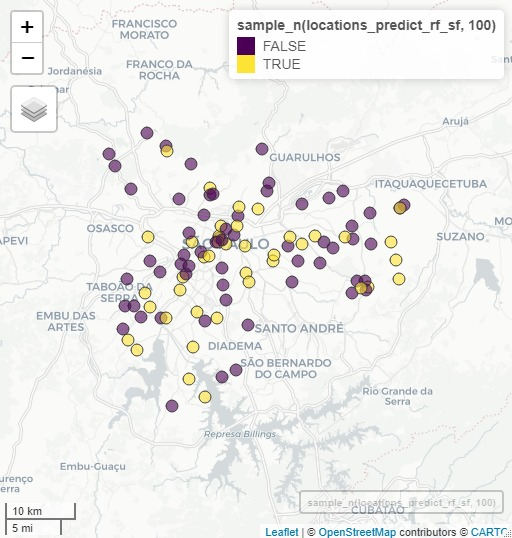
\includegraphics{assets/img/output_rf_viz.jpeg}
\caption{Resultados RF}
\end{figure}

\hypertarget{regressuxe3o-loguxedstica-multinomial}{%
\section{Regressão Logística Multinomial}\label{regressuxe3o-loguxedstica-multinomial}}

Partindo para a regressão logística multinomial, obtemos resultados piores em termos de acerto, verificando-se uma queda de aproximadamente 4\%. As demais conclusões são semelhantes às obtidas através da Random Forest - assim, concluímos que a Random Forest performou melhor na comparação.

\begin{verbatim}
FALSE # A tibble: 2 x 3
FALSE   .metric  .estimator .estimate
FALSE   <chr>    <chr>          <dbl>
FALSE 1 accuracy multiclass     0.326
FALSE 2 kap      multiclass     0.101
\end{verbatim}

\begin{verbatim}
FALSE # A tibble: 2 x 3
FALSE   .metric  .estimator .estimate
FALSE   <chr>    <chr>          <dbl>
FALSE 1 accuracy multiclass    0.327 
FALSE 2 kap      multiclass    0.0953
\end{verbatim}

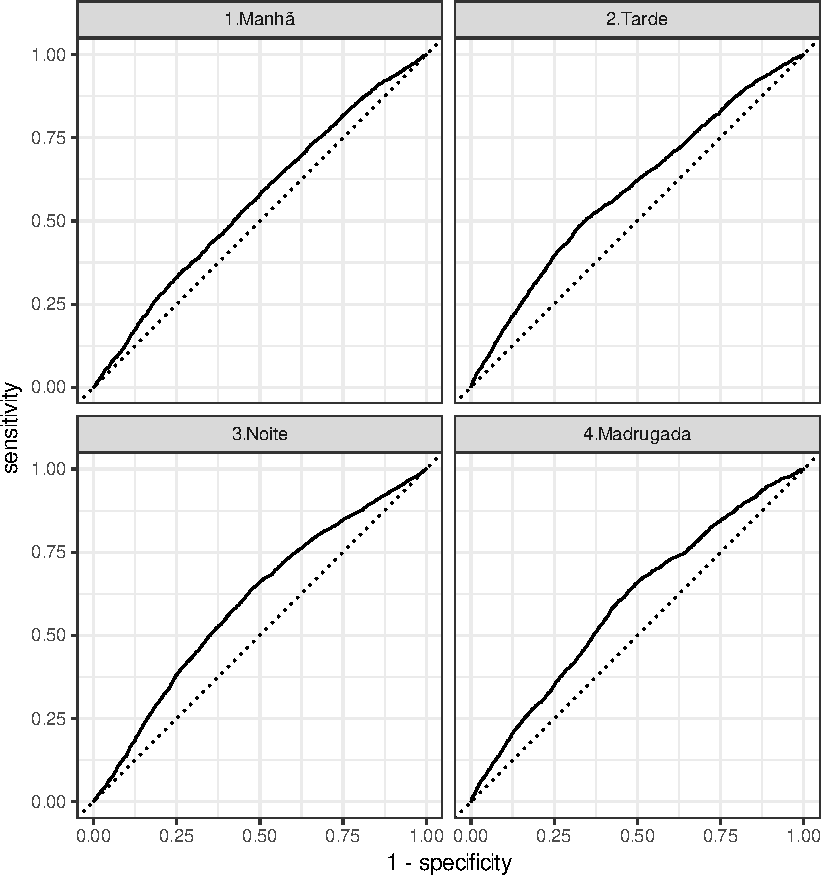
\includegraphics{relatorio_final_files/figure-latex/item Regressao-1.pdf}

\begin{verbatim}
FALSE .
FALSE 4.Madrugada     1.Manhã     2.Tarde     3.Noite 
FALSE  0.32226667  0.04333333  0.30933333  0.32506667
\end{verbatim}

\hypertarget{vizinhos-mais-pruxf3ximos-knn}{%
\section{Vizinhos mais próximos (KNN)}\label{vizinhos-mais-pruxf3ximos-knn}}

Considerando as características de geolocalização dos dados (em especial as variáveis de longitude e latitude), o uso da técnica de vizinhos mais próximos (KNN) pode fornecer interpretações e resultados interessantes. O ajuste aos dados realizado abaixo indica que o método traz um ganho considerável em relação aos até então descritos, com uma acurácia maior que 50\%.

O ajuste da mesma técnica foi feito, também, utilizando apenas as duas variáveis espaciais; o resultado obtido também é interessante, pois resultou em acertos próximos a 50\% mesmo com a redução das variáveis consideradas.

\begin{Shaded}
\begin{Highlighting}[]
\NormalTok{knn\_train\_predict }\OtherTok{\textless{}{-}}\NormalTok{ class}\SpecialCharTok{::}\FunctionTok{knn}\NormalTok{(}\AttributeTok{train=}\FunctionTok{as.matrix}\NormalTok{(dplyr}\SpecialCharTok{::}\FunctionTok{select}\NormalTok{(crime\_training, }\SpecialCharTok{{-}}\FunctionTok{c}\NormalTok{(target))),}
                               \AttributeTok{test=} \FunctionTok{as.matrix}\NormalTok{(dplyr}\SpecialCharTok{::}\FunctionTok{select}\NormalTok{(crime\_training, }\SpecialCharTok{{-}}\FunctionTok{c}\NormalTok{(target))),}
                               \AttributeTok{cl =}  \FunctionTok{as.matrix}\NormalTok{(dplyr}\SpecialCharTok{::}\FunctionTok{select}\NormalTok{(crime\_training,  }\FunctionTok{c}\NormalTok{(target))),}
                               \AttributeTok{k =} \DecValTok{5}\NormalTok{)}
\NormalTok{knn\_test\_predict }\OtherTok{\textless{}{-}}\NormalTok{ class}\SpecialCharTok{::}\FunctionTok{knn}\NormalTok{(}\AttributeTok{train=}\FunctionTok{as.matrix}\NormalTok{(dplyr}\SpecialCharTok{::}\FunctionTok{select}\NormalTok{(crime\_training, }\SpecialCharTok{{-}}\FunctionTok{c}\NormalTok{(target))),}
                              \AttributeTok{test=} \FunctionTok{as.matrix}\NormalTok{(dplyr}\SpecialCharTok{::}\FunctionTok{select}\NormalTok{(crime\_testing, }\SpecialCharTok{{-}}\FunctionTok{c}\NormalTok{(target))),}
                              \AttributeTok{cl =} \FunctionTok{as.matrix}\NormalTok{(dplyr}\SpecialCharTok{::}\FunctionTok{select}\NormalTok{(crime\_training, }\FunctionTok{c}\NormalTok{(target))),}
                              \AttributeTok{k =} \DecValTok{5}\NormalTok{)}
\NormalTok{crime\_training}\SpecialCharTok{$}\NormalTok{acerto }\OtherTok{\textless{}{-}}\NormalTok{ (crime\_training}\SpecialCharTok{$}\NormalTok{target }\SpecialCharTok{==}\NormalTok{ knn\_train\_predict)}
\NormalTok{crime\_training}\SpecialCharTok{$}\NormalTok{acerto }\SpecialCharTok{\%\textgreater{}\%}\NormalTok{ table }\SpecialCharTok{\%\textgreater{}\%}\NormalTok{ prop.table}
\NormalTok{crime\_testing}\SpecialCharTok{$}\NormalTok{acerto }\OtherTok{\textless{}{-}}\NormalTok{ (crime\_testing}\SpecialCharTok{$}\NormalTok{target }\SpecialCharTok{==}\NormalTok{ knn\_test\_predict)}
\NormalTok{crime\_testing}\SpecialCharTok{$}\NormalTok{acerto }\SpecialCharTok{\%\textgreater{}\%}\NormalTok{ table }\SpecialCharTok{\%\textgreater{}\%}\NormalTok{ prop.table}
\NormalTok{crime\_testing }\OtherTok{\textless{}{-}}\NormalTok{ crime\_testing[, }\SpecialCharTok{{-}}\DecValTok{23}\NormalTok{]}
\NormalTok{crime\_training }\OtherTok{\textless{}{-}}\NormalTok{ crime\_training[, }\SpecialCharTok{{-}}\DecValTok{23}\NormalTok{]}
\end{Highlighting}
\end{Shaded}

\begin{verbatim}
FALSE # A tibble: 2 x 2
FALSE   .         n
FALSE   <chr> <dbl>
FALSE 1 FALSE 0.366
FALSE 2 TRUE  0.634
\end{verbatim}

\begin{verbatim}
FALSE # A tibble: 2 x 2
FALSE   .         n
FALSE   <chr> <dbl>
FALSE 1 FALSE 0.426
FALSE 2 TRUE  0.574
\end{verbatim}

\begin{figure}
\centering
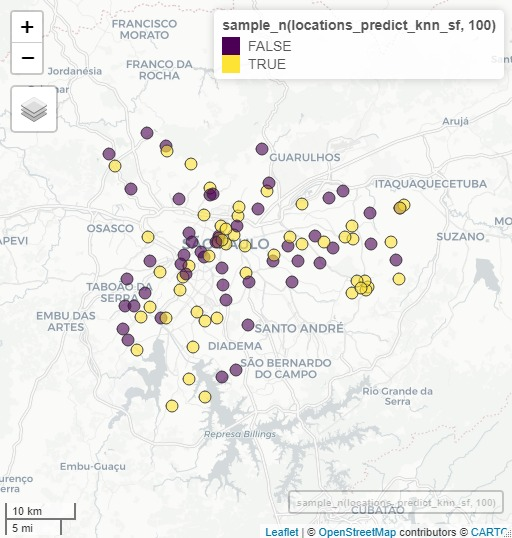
\includegraphics{assets/img/output_knn_viz.jpeg}
\caption{Resultados KNN}
\end{figure}

\hypertarget{xgboost-1}{%
\section{XGBoost}\label{xgboost-1}}

Outro modelo de machine learning foi proposto para a modelagem do nosso problema. O XGBoost é um método baseado em árvores e este modelo foi proposto em 2016 no paper ``Xgboost: A Scalable Tree Boosting System''. Para tunarmos os parâmetros do modelo, separamos a amostra de treino em duas, a fim de escolhermos o melhor conjunto de parâmetros para o nosso modelo. Mesmo assim, com os parâmetros escolhidos baseados em um grid não foi possível alcançar uma acurácia melhor do que a do KNN para a base out-of-sample.

\begin{verbatim}
FALSE [1] "Final Accuracy = 34.17%"
\end{verbatim}

\hypertarget{conclusao}{%
\chapter{Conclusão}\label{conclusao}}

Como apresentado na seção anterior, a métrica acurácia indica que métodos baseados em árvore ou regressão atingiram um acerto na casa de 30\%, enquanto o KNN, principalmente devido às variáveis bastante precisas de latitude e longitude, alcança resultados superiores a 50\% de acerto.

Em relação às possíveis aplicações práticas que possam ser de interesse a partir desta base de dados, concluímos que a questão espacial do problema - isto é, localização da ocorrência - é de grande relevância para obter relações com o horário da mesma. Somando esta conclusão à interpretabilidade do KNN, que se baseia justamente em distâncias entre as variáveis, este trabalho mostra que há espaço para utilização destas informações para melhorias em políticas públicas para segurança.

\hypertarget{referuxeancias}{%
\chapter*{Referências}\label{referuxeancias}}
\addcontentsline{toc}{chapter}{Referências}

\hypertarget{refs}{}
\begin{CSLReferences}{1}{0}
\leavevmode\hypertarget{ref-breiman1996}{}%
BREIMAN, Leo. 1996. \emph{Bagging predictors. Machine learning}.

\leavevmode\hypertarget{ref-breiman2001}{}%
---------. 2001. \emph{Random forests. Machine learning}.

\leavevmode\hypertarget{ref-friedman2002}{}%
FRIEDMAN, Jerome H. 2002. \emph{Stochastic gradient boosting}.

\leavevmode\hypertarget{ref-hearst1998}{}%
HEARST, Marti A. et al. 1998. \emph{Support vector machines. IEEE Intelligent Systems and their applications}.

\leavevmode\hypertarget{ref-svozil1997}{}%
VOZIL, Vladimir; POSPICHAL, Daniel; KVASNICKA. 1997. \emph{Introduction to multi-layer feed-forward neural networks}.

\end{CSLReferences}

\end{document}
